\hypertarget{sec:sota}{%
\chapter{State of the Art}\label{sec:sota}}

The following analysis of migration methods is focused on dedicated \gls{Web Migration} approaches, i.e. methods that move \glspl{Legacy System} to a \glslink{web}{Web}-based target environment.
For that, this chapter
\begin{itemize}
\item introduces relevant standards and a migration reference model as basis for the description of \gls{Web Migration} approaches,
\item assesses \gls{Web Migration} approaches according to the requirements,
\item analyzes assessment results from several group and cross-cutting perspectives, and
\item identifies shortcomings of existing \gls{Web Migration} approaches to be addressed by this thesis.
\end{itemize}

The topic of \gls{Web Migration} is located in the overlap of two major areas of research: \gls{Web Engineering} and \gls{Software Migration}.
It requires profound knowledge from both areas to successfully plan and conduct a \gls{Web Migration}.
Knowledge of \gls{web} paradigms, architectures, technologies, and development processes is required due to the specific characteristics of the \gls{web} as target platform of the migration.
Knowledge of \glspl{Legacy System}, migration strategies, \gls{Reverse Engineering}, and migration planning is required due to the specific characteristics of \glspl{Legacy System} and different nature of migration activities.
Thus, isolated consideration of approaches from either only \gls{Web Engineering} or \gls{Software Migration} is not sufficient.

Dedicated \emph{\gls{Web Engineering} approaches} such as \gls{webml}/ \gls{ifml} \autocite{OMG2015IFML}, UWE \autocite{Koch2008UWE}, AWE \autocite{McDonald2005AWE} or OOHDM \autocite{Schwabe1996OOHDM} fail to address any \gls{Web Migration} aspects beyond \gls{Forward Engineering} (in particular requirements \cref{s:1} and \cref{c:2}).
Most \gls{Web Engineering} approaches start from scratch, not from an existing \gls{Legacy System} (cf.~\emph{brownfield software development} \autocite{Hopkins2008Brownfield}) which requires a different set of methods, e.g.~requirements elicitation instead of re-discovery of requirements.
\emph{Generic \gls{Software Migration} and \glslink{Software Modernization}{Modernization} approaches} such as Chicken Little \autocite{Brodie1995Migrating}, Butterfly \autocite{BingWu1997Butterfly}, XIRUP\autocite{Fuentes-Fernandez2012XIRUP} or Renaissance \autocite{Warren2002Renaissance} fail to address the specific characteristics of the \gls{web} as target platform (requirement S2).

The selection of approaches assessed in the following analysis is based on their orientation towards the thesis' overarching research question RQ1 and the availability of published research results within \gls{Web Engineering} and \gls{Software Migration} communities.
Suitability of the assessed approaches for supporting \glspl{isv} to commence a \gls{Web Migration} is evaluated employing the requirements and evaluation scheme introduced in the previous chapter.


\vspace{-15pt}
\hypertarget{standards-and-reference-models}{%
\section{Standards and Reference Model}\label{standards-and-reference-models}}
\vspace{15pt}

This section provides a brief introduction to relevant standards and reference models from the fields of \gls{Software Modernization} and software migration.
The standards represent the technological basis of many \gls{Web Migration} approaches, and the Horseshoe model is the conceptual standard model of \gls{Reengineering} approaches.
The reference model for software migration provides a common basis for description of the assessed approaches and the solution presented in this thesis.

\vspace{-10pt}
\hypertarget{sec:adm}{%
\subsection{Architecture-Driven Modernization (ADM)}\label{sec:adm}}
\vspace{10pt}

Extending \gls{mda} \autocite{OMG2014MDA} principles to \gls{Software Modernization}, \gls{adm} provides a family of related \gls{omg}\footnote{\url{https://www.omg.org/} Retrieved: 6.12.2019} standards\footnote{cf.~\url{https://www.omg.org/spec/category/software-modernization}} that form the technological basis of many \gls{Web Migration} approaches assessed in this chapter.
\gls{adm} specifies a process of understanding and evolving existing software assets for migration, restructuring, refactoring, translation to other languages, and porting.
The \gls{adm} Horseshoe\footnote{adapted from the original SEI horseshoe reengineering model \autocite{Kazman1998Horseshoe}} Model \autocite{Perez-Castillo2011KDM,Perez-Castillo2011MARBLE,Khusidman2007} is the standard model of most \gls{Reengineering} approaches.
As shown in \cref{fig:adm-horseshoe-a}, it consists of three stages: \gls{Reverse Engineering}, restructuring, \gls{Forward Engineering}, embedded into a standards-based model-driven methodology.
These stages consider \glslink{Software Modernization}{modernization} in the business and IT domain on the three architectural levels: business architecture, application/data architecture, technical architecture \autocite{OMG2008ADMWhitepaper}.
\Cref{fig:adm-horseshoe-b} shows \gls{adm} standards used at different levels and stages in the \gls{adm} Horseshoe.
The following paragraphs briefly summarize the four most relevant standards which have been observed in use in various \gls{Web Migration} methods in the subsequent state of the art analysis, as indicated in \cref{tbl:adm-usage}.
%The \gls{admtf} advocates a standards-based model-driven methodology for modernizing existing applications on all three architectural levels.
\begin{figure}[hbt]
\hypertarget{fig:adm-horseshoe-a}{%
\centering%
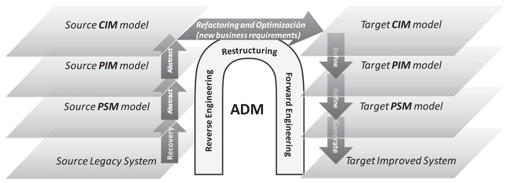
\includegraphics[width=0.98\textwidth]{../figures/adm_horseshoe_1.png}%
\caption[Model-Driven Reengineering in the ADM Horseshoe Model]{Model-Driven Reengineering in the ADM Horseshoe Model \autocite{Perez-Castillo2011MARBLE}}%
\label{fig:adm-horseshoe-a}%
}
\end{figure}
\begin{figure}[hbt]
\hypertarget{fig:adm-horseshoe-b}{%
\centering%
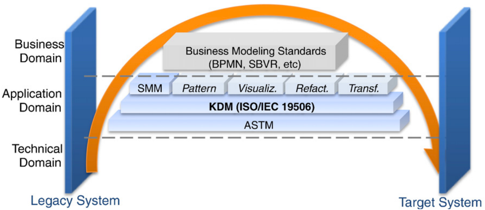
\includegraphics[width=0.98\textwidth]{../figures/adm_horseshoe_2.png}%
\caption[ADM standards in the ADM Horseshoe Model]{ADM standards in the ADM Horseshoe Model \autocite{Perez-Castillo2011KDM}}%
\label{fig:adm-horseshoe-b}%
}
\end{figure}

\textbf{Knowledge Discovery Metamodel (KDM)} \autocite{OMG2016KDM} is the central \gls{adm} standard, around which the other \gls{adm} standards are defined \autocite{Perez-Castillo2011KDM} and
was adopted as \gls{iso}/\gls{iec} 19506:2012 standard\footnote{\url{https://www.iso.org/standard/32625.html} Retrieved: 6.12.2019}.
The usage of \gls{kdm} in this thesis is based on version 1.4 of September 2016.
\gls{kdm} specifies a conceptual model for the representation of knowledge in \glspl{Legacy System} and its mapping onto \gls{xml}-based \gls{omg} standards such as \gls{mof}\footnote{\url{https://www.omg.org/spec/MOF/} Retrieved: 6.12.2019} and \gls{xmi}\footnote{\url{https://www.omg.org/spec/XMI/} Retrieved: 6.12.2019}, allowing integration and interoperability across \gls{Software Modernization} tools.
The \gls{kdm} \gls{metamodel} is a \gls{mof}-compliant Entity-Relationship model, describing physical \glspl{artifact} of a \gls{Legacy System} (e.g.~source files, executables), code elements (e.g.~modules, classes, interfaces), control-flow and data-flow relationships (read/write, call, exceptions), runtime resources (e.g.~relational tables, events, processes) and abstractions (e.g.~conceptual roles, flows, relationships).
\gls{kdm} provides an ontology of \glspl{Legacy System} \autocite{Perez-Castillo2011KDM} describing \glspl{Legacy System} at a granularity above procedure level.
Throughout this thesis, mappings to \gls{kdm} are provided in order to clarify the semantics of the terms used and facilitate interoperability by providing in brackets the identifier of the \gls{kdm} concept preceded by the word \gls{kdm} and a colon.
For instance, (\gls{kdm}: \emph{SourceFile}) is to be understood as a shorthand to refer to the SourceFile concept in \gls{kdm} 1.4 \autocite{OMG2016KDM}.

\textbf{\gls{astm}} \autocite{OMG2011ASTM} is a complementary \gls{adm} standard to \gls{kdm}.
Combined with \gls{kdm}, it provides a universal software modeling framework, adding the capability of describing \glspl{Legacy System} at a granularity below procedure level used by several model-driven \gls{Web Migration} approaches for low-level software models.
%by providing a mapping of all code-level programming language statements into low-level software models.
To achieve high applicability for any programming language, the syntax is represented using \emph{\glspl{ast}}, a hierarchical representation of all abstract source code constructs.
\gls{astm} defines a \gls{gastm} using \gls{mof}-compliant \gls{uml} \autocite{OMG2017UML}, that allows specifying \glspl{pim} of \glspl{ast}.
The \glspl{psm} for various programming languages are supported through the \gls{sastm} extensions.

\textbf{\gls{smm}} \autocite{OMG2012SMM} specifies a \gls{metamodel} for representing measurement information related to structured information models, in particular MOF-compliant models.
It addresses the need for \gls{Web Migration} metrics in combination with \gls{kdm}/\gls{astm}.
\gls{smm} allows to define measures in terms of basic calculation concepts (counts, mathematic operators, averages) as well as pre-defined metrics (e.g.~cyclomatic complexity, \gls{loc}), observations including metadata (e.g.~provenience, creation time) and measurements (results of the application of measures to observations).
Measurements are applicable to any \gls{kdm}/\gls{astm} element, allowing to represent characteristics of \glspl{Legacy System} such as maintainability index \autocite{Coleman1994MaintainabilityIndex}.
\gls{smm}'s conceptual model of construction of metrics based on computable measures is used in the \gls{Web Migration} solution presented in this thesis in the area of user interface similarity.

\textbf{\gls{mof} \gls{qvt}} \autocite{OMG2016QVT} specifies model-to-model \glspl{Transformation} in highly model-driven \gls{Web Migration} approaches.
In the \gls{adm} horseshoe, it connects the source and target models as well as models of different levels of abstraction (\gls{psm}/\gls{pim}/\gls{cim}) through \glspl{Transformation}.
Queries are formal expressions to select parts of a model; views are complex queries which allow selecting complex model subsets; \glspl{Transformation} define mappings from one model to another and make use of queries and views.
\gls{qvt} defines two basic types of \gls{Transformation} languages: \gls{qvt}-relational and \gls{qvt}-operational.
\gls{qvt}-relational are declarative languages and support bi-directional \gls{Transformation}, whereas \gls{qvt}-operational are imperative languages for unidirectional \glspl{Transformation}.
For both types, the \gls{qvt} standard specifies a concrete \gls{Transformation} language: the Relations language QVTr and the Operational Mappings language QVTo.
%QVTr is the \gls{qvt} Relations language, specifying symmetric relationships between \gls{mof}-compliant models and supporting complex object pattern matching in a declarative way.
%QVTo is the Operational Mappings language defined by \gls{qvt} and supports \glspl{Transformation} through a procedural style of defining mappings from one model to another.
%The \gls{qvt} languages employ OCL\footnote{\url{https://www.omg.org/spec/OCL/} Retrieved: 6.12.2019} as expressions language.
\gls{qvt}'s conceptual model of queries on the \glslink{Legacy System}{legacy} for \gls{Transformation} is used in the \gls{Web Migration} solution presented in this thesis for integration with model-driven approaches through queriable external representations of discovered knowledge in the \gls{Legacy System}.

\hypertarget{tbl:adm-usage}{}
\begin{table}[h!]
  \caption{Usage of ADM standards in \gls{Web Migration} methods}
  \label{tbl:adm-usage}
  \centering
    \begin{tabularx}{0.98\linewidth}{ XXXXX } 
    \toprule
    \textbf{ADM} & \textbf{KDM} & \textbf{ASTM} & \textbf{SMM} & \textbf{QVT}\\
    \midrule
    
   REMICS, PRECISO, CloudMIG, L2CMH, MIGRARIA, serviciFi & ARTIST, REMICS, CloudMIG, MIGRARIA & ARTIST, REMICS, MIGRARIA & ARTIST, REMICS, CloudMIG & PRECISO, MIGRARIA\\
    \bottomrule
    \end{tabularx}
\end{table}


\vspace{-20pt}
\hypertarget{remip}{%
\subsection{Reference Migration Process}\label{remip}}

Sneed et al.~introduced a reference model for software migration, the Reference Migration Process (\gls{remip}) \autocite{Sneed2010ReMiP,Gipp2007ReMiP} based on a synthesis of existing software evolution and software development methods.
Requirements \cref{s:1} and \cref{c:4} are specified against its Phases and Disciplines.
It serves as generic and adaptable framework for understanding and describing arbitrary \gls{Web Migration} processes assessed in the following analysis.
The \gls{Web Migration} solution presented in this thesis is described using \gls{remip} taxonomy and proposed methods are mapped to \gls{remip} disciplines in order to use the established software migration semantics and facilitate the integration of the proposed methods with other \gls{Web Migration} approaches.
The following paragraph outlines the main aspects of \gls{remip}.
\begin{figure}[hbt]
\hypertarget{fig:remip}{%
\centering%
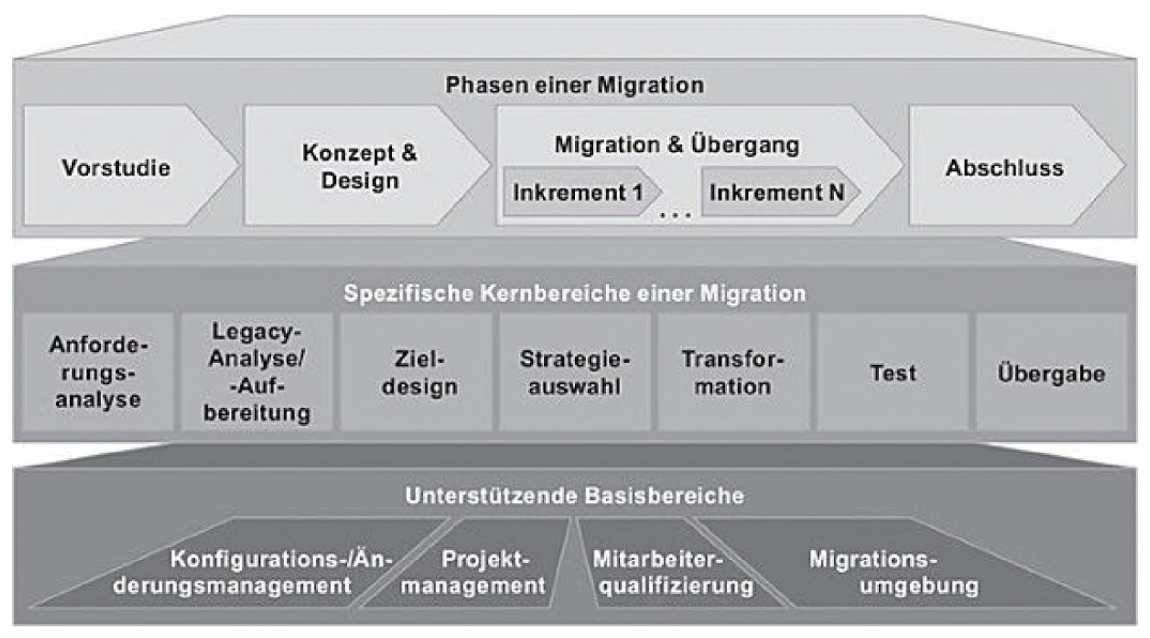
\includegraphics[width=0.98\textwidth]{../figures/remip.pdf}%
\caption[\gls{remip} Overview]{\gls{remip} Overview \autocite[adapted from][]{Sneed2010ReMiP}}\label{fig:remip}%
}
\end{figure}\vspace{-10pt}

A software migration is considered as a project, and \gls{remip}'s focus is on the management perspective of this project.
\gls{remip} structures relevant activities according to temporal and logical aspects (cf.~\cref{fig:remip}).
From the temporal perspective, activities are assigned to \emph{migration phases}.
From the logical perspective, activities are grouped into migration-specific \emph{core disciplines} and cross-cutting supporting \emph{base disciplines}.
\gls{remip} distinguishes four phases: \emph{Preliminary Study}, which comprises technical, economical and organizational feasibility analysis, \emph{Conceptualization and Design}, addressing migration planning activities such as legacy analysis, strategy selection, and target architecture specification, \emph{Migration and Transition}, conducting iterative package-wise \gls{Transformation}, testing and delivery, and \emph{Closing down}, comprising activities to archive project documentation and ensure continuous operation of the migrated system.
%Each phase is terminated by a milestone which serves as a decision point whether to continue the migration.
%These four milestones are: project objective \& process recommendation, binding master plan, migrated system release and final documentation.
The migration-specific core disciplines are \emph{requirements analysis}, \emph{legacy analysis}, \emph{target design}, \emph{strategy selection}, \emph{implementation}, \emph{test} and \emph{deployment} and represent activities from (forward) software engineering extended for migration (e.g.~requirements analysis or target design) as well as activities intrinsic to the migration domain (e.g.~legacy analysis or strategy selection).
The core disciplines are supported by base disciplines addressing cross-cutting activities to provide the operational context of the migration project. %: \emph{configuration \& change management}, \emph{project management}, \emph{staff qualification} and \emph{migration environment}.
%The holistic view of the \gls{remip} reference model provides a framework for understanding the context of software migration and thus \gls{Web Migration}.
%The definition of requirement \cref{s:1} refers to the \gls{remip} phases.
%In \cref{tbl:awsm-remip} we provide mappings of the solutions provided in this thesis to \gls{remip} phases and disciplines.

\vspace{-15pt}
\hypertarget{sec:approaches}{%
\section{Web Migration Approaches}\label{sec:approaches}}
\vspace{15pt}

This section surveys the state of the art of \gls{Web Migration} approaches.
It is organized into four groups:
\begin{itemize}
\tightlist
\item
  \textbf{\gls{soa}} migration approaches
\item
  \textbf{Cloud} migration approaches
\item
  \textbf{\gls{Web Systems Evolution}} approaches
\item
	\textbf{\gls{Web Application}} migration approaches
\end{itemize}
These groups are defined by the \emph{target environment} (\gls{soa}, Cloud, \gls{Web Application}) and \emph{source system} (\gls{Web Systems Evolution}) and represent the common classification based on areas of interest in \gls{Web Migration} research  \autocite{Kienle2014EvolutionWeb}.
We confirmed these groups in our systematic mapping study \autocite{Heil2017Survey} which serves as the basis for this state of the art analysis.
While the scope of this previous survey was wider, comprising 122 primary studies and tools resulting from inclusion/exclusion criteria-based study selection from 870 initial search results from queries and snowballing across six data sources including dedicated methods and tools for specific migration disciplines (cf.~\gls{remip}), the following 22 approaches represent a condensed and updated overview of the state of the art of \gls{Web Migration} in 2019, focusing on comprehensive approaches with high \emph{migration discipline coverage} (cf.~\autocite{Heil2017Survey}), multi-publication approaches and larger-scale research projects.

The characteristics of individual approaches within the same group, however, differ significantly.
In our Survey \autocite{Heil2017Survey}, we observed that this is partially rooted in the different overall methodologies which they use.
These form independent dimensions of description of migration approaches, which are orthogonal to the four groups introduced above.
We identified three main methodology groups:

\begin{itemize}
\tightlist
\item
  \textbf{\gls{Encapsulation}} approaches, that wrap the unchanged \gls{Legacy System} or parts of it and expose a new interface \autocite[cf.~to \emph{external interface}, \emph{internal implementation} in \emph{encapsulation} definition][]{ISO/IEEE24765Vocabulary} which is then integrated with the \gls{target system},
\item
  \textbf{\gls{Reengineering}} approaches, that employ \emph{reverse engineering} techniques to extract information from the \gls{Legacy System} and follow up with \emph{forward engineering} to create the \gls{target system} \autocite[cf.~also to \gls{iso}/\gls{ieee} reengineering definition in][]{ISO/IEEE24765Vocabulary,IEEE1219Maintenance} and
\item
  \textbf{\gls{Transformation}} approaches, that process the \glslink{Legacy System}{legacy} source code by a series of \emph{automatic steps} turning it into the \gls{target system}'s source code.
\end{itemize}

\hypertarget{tbl:sota-groups}{}
\begin{table}[h]
  \caption[Overview of assessed web migration approaches]{Overview of web migration approaches with regard to
research areas/target architectures and methodologies}
  \label{tbl:sota-groups}
  \centering
    \begin{tabularx}{0.98\linewidth}{ XXXXX } 
    \toprule
    & \textbf{Encaps.} & \textbf{Reeng.} & \textbf{Transform.} & \textbf{Other}\\
    \midrule
    \textbf{SOA} & PRECISO, Marchetto2008, Gaps2Ws & serviciFi & SOAMIG, SAPIENSA & SMART\footnotemark\\
    \textbf{Cloud} & AMS, NCHC & IC4 & REMICS, L2CMH, ARTIST, CloudMIG & AWS Migration\footnotemark\\
    \textbf{WSE} & & & MIGRARIA, MigraSOA &\\
    \textbf{Web Application} & MELIS, M\&S SW, CelLEST, DAS & UWA/UWAT+ & TUIMigrate &\\
    \bottomrule
    \end{tabularx}
\end{table}
\addtocounter{footnote}{-1}
\footnotetext{addresses only phases before migration}
\addtocounter{footnote}{1}
\footnotetext{migration planning framework without concrete encapsulation/reengineering/transformation methodology}

\Cref{tbl:sota-groups} provides an overview of the approaches assessed in this section in the two grouping schemes \emph{research areas and target architectures} and \emph{methodologies}.

%A more comprehensive overview of Reengineering technologies can be found in \autocite{Perez-Castillo2011Reengineering}.

The following subsections report on corresponding approaches in terms of their name, related publications, research project, overall aim, main focus, method, and evaluation results according to the requirements introduced in \cref{sec:requirements}. The following symbols represent the ratings according to the three-level assessment scheme introduced in \ref{sec:requirements}: \Circle : not satisfied, \LEFTcircle : partially satisfied, \CIRCLE : satisfied.

\vspace{-10pt}
\hypertarget{sec:soa-migration}{%
\subsection{Migration to SOA}\label{sec:soa-migration}}
\vspace{10pt}

\emph{Web Services} are one of the major target environments of \gls{Web Migration}.
Web Services are often implemented as either \gls{rest} \autocite{Fielding2017REST} Web Service, or as SOAP\footnote{\url{https://www.w3.org/TR/soap/} Retrieved: 6.12.2019} service, typically with a \gls{wsdl} service interface description and SOAP over \gls{http} communication \autocite{Lewis2008SMART}.
A significant share of \gls{Web Migration} research is on migration to Web Services, with the goal to ``reengineer the \glspl{Legacy System} into a set of services which can be dynamically selected and are distributed across organization boundaries'' \autocite{Razavian2014a}.
We employ the term \emph{\gls{soa} migration} to refer to the entire range of \gls{Web Migration} towards SOAP and REST \gls{web} Services in both the federated \gls{soa} application integration and smaller-grained services architectural perspective for maintaining naming consistency with existing research \autocite{Khadka2013SurveySOAMigration,Razavian2011SOASurvey,Almonaies2010SOAStrategies} that addresses migration to Web Services.

%Service Oriented Architectures are one of the major target environments of \gls{Web Migration}.
%\gls{soa} is a business-driven approach that abstracts software by decomposition into loosely-coupled services enabling to address rapidly changing business needs through reuse of existing software assets \autocite{Gold2004SOA}.
%A \emph{\gls{soa} service} is a ``coarse-grained, discoverable, and self- contained software entity that interacts with applications and other services through a loosely coupled, often asynchronous, message-based communication model'' \autocite{Lewis2005SMART}.
%\gls{soa} migration research focuses on \glspl{target system} that adhere to the fine-grained \gls{soa} notion of \emph{microservices} -- i.e.~one application composed of a set of small services -- rather than on integrating several applications through services to build federated applications.
%However, the term microservices was coined much later, and since it is commonly used in literature, 

%we employ the term \emph{\gls{soa} migration} to describe the entire range of migration towards \gls{web} services SOAP and REST in both the federated \gls{soa} and microservices flavor.
%For more details on \gls{soa} migration refer to the dedicated surveys \autocite{Khadka2013SurveySOAMigration,Razavian2011SOASurvey,Almonaies2010SOAStrategies}.

\hypertarget{smart}{%
\subsubsection*{SMART}\label{smart}}

CMU SEI's SMART method \autocite{Lewis2008SMART,Lewis2005SMART} initially published in 2005 as Service Migration and Reuse Technique is a decision-making and planning approach for the migration of \glslink{Legacy System}{legacy} components to services.
SMART provides a process for legacy analysis, service identification and definition of the target \gls{soa} environment, a service migration interview guide (SMIG), a tool for automating data collection from SMIG and \gls{artifact} templates for various analysis results.
The iterative SMART process starts with establishing the migration context, including analysis of business and technical context, stakeholder analysis, \gls{Legacy System} understanding and service identification following a top-down -- based on business and mission goals and processes -- and bottom-up -- based on existing \glslink{Legacy System}{legacy} functionality -- approach resulting in a business process to service mapping.
Great emphasis is put on the migration feasibility decision, taking into account migration potential according to a set of proposed determinations.
A subset of candidate services is identified and specified in further detail, information about the \gls{Legacy System} is gathered in more detail through interviews with technical staff, and the target \gls{soa} environment is defined.
Gap analysis is used to provide estimates of cost, risk, and effort to migrate the candidate service to the target \gls{soa} environment.
All information gathered in the previous activities feeds into the definition of the migration strategy that can include a pilot project, migration guidelines, migration path (\gls{Encapsulation}, \gls{Transformation}, \gls{Reengineering}), etc.
Based on experience in applying SMART, SEI realized that many organizations were not ready, did not know enough about \gls{soa} to consider migration or had not identified a particular system to migrate, so the scope of SMART was extended along with a redefinition of the acronym to \gls{soa} Migration, Adoption, and Reuse Technique \autocite{Lewis2010SMART}.
In its extended version\footnote{based on the 2013 SMART materials available at \url{https://resources.sei.cmu.edu/library/asset-view.cfm?assetid=508038}}, the original SMART method is now one of five variations of the SMART process, which form a family of related techniques addressing different organizational needs.
SMART-MP (migration pilot) represents the original perspective, SMART-AF (adoption feasibility) supports organizations' decision making whether to migrate to \gls{soa}, SMART-ESP (enterprise service portfolio) supports to select from several \glspl{Legacy System} which parts to expose as services, SMART-ENV (\gls{soa} environment) supports building the required \gls{soa} infrastructure and SMART-SYS (Service-Oriented Systems Development) combines all of the before mentioned variations.
SMART has influenced following migration approaches such as REMICS \autocite{REMICS2013Handbook,Mohagheghi2011REMICS}.

SMART in all variations has a dedicated focus on phases prior to migration but does not include communication of necessity and benefits of the migration, half-satisfying requirement \cref{s:1}.
It is designed for migration to \gls{soa}-based \glspl{Web System}, \glslink{web}{Web}-based user interfaces are not considered achieving half fulfillment for \cref{s:2}.
\Cref{c:1} is prominently addressed, including basic techniques like feasibility assessment, incremental activities updating \glspl{artifact} and incremental process as well as migration pilots.
Regarding \cref{c:2}, data about cost, risk, and effort are gathered contributing to the \gls{business case} and relevant knowledge is captured from the \gls{Legacy System}.
SMART enables reuse of functionality, but not user interaction, yielding half fulfillment for \cref{c:2}.
Expertise requirements (\cref{c:3}) for SMART are not high due to the straightforward, well-defined process and activities and the tools and templates guiding each step.
Integration into ongoing development is described neither on process nor \gls{artifact} level, leaving \cref{c:4} unaddressed.

\hypertarget{tbl:SMART-eval}{}
\begin{longtable}[]{@{}llllll@{}}
\caption{\label{tbl:SMART-eval}SMART Evaluation}\tabularnewline
\toprule
\cref{s:1} Initial & \cref{s:2} Web & \cref{c:1} Risk & \cref{c:2} Reuse & \cref{c:3} Exp & \cref{c:4} Agile\tabularnewline
\midrule
\endfirsthead
\toprule
\cref{s:1} Initial & \cref{s:2} Web & \cref{c:1} Risk & \cref{c:2} Reuse & \cref{c:3} Exp & \cref{c:4} Agile\tabularnewline
\midrule
\endhead
\LEFTcircle & \LEFTcircle & \CIRCLE & \LEFTcircle & \CIRCLE & \Circle\tabularnewline
\bottomrule
\end{longtable}

\hypertarget{sapiensa}{%
\subsubsection*{SAPIENSA}\label{sapiensa}}

SAPIENSA (Service-enAbling Pre-exIsting ENterpriSe Assets) \autocite{Razavian2010SAPIENSA,Razavian2013PHD,Razavian2012,Razavian2014a,Razavian2009} is a \gls{soa} migration research project\footnote{\url{https://www.nwo.nl/en/research-and-results/research-projects/i/19/4019.html} Retrieved: 6.12.2019} under the Dutch Joint Academic and Commercial Quality Research and Development (Jacquard) program on Software Engineering. In the context of SAPIENSA, Razavian et al.~developed a \gls{soa} migration method based on knowledge management focusing on a rational investigation of \glslink{Legacy System}{legacy} assets as candidate services, isolation of their properties and \gls{Transformation} into business services.
SAPIENSA results also contributed to EU FP7 project S-CUBE\footnote{\url{https://cordis.europa.eu/project/reference/215483} Retrieved: 6.12.2019}.
The SAPIENSA method aims at exploiting architectural knowledge to enable the \gls{Transformation} to services on different \emph{\gls{soa} abstraction levels} \autocite{Razavian2010SOA-MF}.
Its focus on knowledge management acknowledges the importance of knowledge in migration projects.

Similar to SMART, SAPIENSA employs a \emph{middle-out} strategy, combining top-down domain and business decomposition with bottom-up \glslink{Legacy System}{legacy} understanding.
The SAPIENSA process consists of three phases: architectural knowledge (AK) elicitation, \gls{Transformation}, and service composition.
The AK elicitation extracts and externalizes problem-related (e.g.~business processes and rules) and solution-related (e.g.~structure, design decisions and rationale) knowledge and identifies candidate services.
\gls{Transformation} is carried out on all levels of abstraction: design elements are reshaped, architecture is restructured, and business models and strategies are altered.
The service composition phase focuses on service-based \gls{Forward Engineering} using the service composition model (SCM) leveraging services obtained from the \gls{Legacy System}, newly developed services, and external services.
Model-driven gap analysis \autocite{Nguyen2009} supports \gls{Transformation} between as-is and to-be parts of AK such as as-is business process portfolio and to-be business process portfolio, identifying discrepancies and identifying realization strategies.
These strategies enable decision making about re-using or re-structuring \glslink{Legacy System}{legacy} assets or re-developing them and serve as input to lower-level service \gls{Transformation}.
The SAPIENSA approach has been elaborated in the "lean and mean" migration strategy \autocite{Razavian2012,Razavian2014a}, generalizing core migration activities from common industry practices.

SAPIENSA addresses phases prior to migration but does not contribute to communicating necessity and benefits thus half-satisfying \cref{s:1}.
The \gls{target system} is a service-based \gls{Web System}; migration of \gls{gui} is not considered resulting in half fulfillment of \cref{s:2}.
No \gls{risk management} (\cref{c:1}) is proposed.
Reuse of \glslink{Legacy System}{legacy} assets is employed to retain functionality, but user interaction is not considered, which half-satisfies \cref{c:2}.
Since the SAPIENSA process is not bound to sophisticated \gls{Transformation} methods or technologies, expertise requirements are not high, but no supporting tools are provided.
Therefore the criteria for \cref{c:3} are half satisfied.
Integration into ongoing development is not addressed, yielding no fulfillment of \cref{c:4}
SAPIENSA contributed to systematizing research on \gls{soa} migration by producing the conceptual \gls{soa} migration reference framework \gls{soamf} which has contributed to the understanding of migration processes and knowledge in \glspl{Legacy System} of this thesis as described in \cref{sec:formalisms}.

\hypertarget{tbl:SAPIENSA-eval}{}
\begin{longtable}[]{@{}llllll@{}}
\caption{\label{tbl:SAPIENSA-eval}SAPIENSA Evaluation}\tabularnewline
\toprule
S1 Initial & S2 Web & C1 Risk & C2 Reuse & C3 Exp & C4 Agile\tabularnewline
\midrule
\endfirsthead
\toprule
S1 Initial & S2 Web & C1 Risk & C2 Reuse & C3 Exp & C4 Agile\tabularnewline
\midrule
\endhead
\LEFTcircle & \LEFTcircle & \Circle & \LEFTcircle & \LEFTcircle & \Circle\tabularnewline
\bottomrule
\end{longtable}

\hypertarget{servicifi}{%
\subsubsection*{ServiciFi}\label{servicifi}}

The ServiciFi method for \gls{soa} Migration presented by \citet{Khadka2011ServiciFi,Khadka2016PHD} is part of the ServiciFi project\footnote{\url{https://servicifi.wordpress.com} Retrieved: 6.12.2019} which aims at transforming monolithic software of the financial services domain into services to enable the creation of new \gls{soa}-based applications.
As typical for \gls{soa} migration approaches, it focuses on service identification, extraction, and \gls{Transformation}.
The ServiciFi method itself was created using method engineering to assemble method fragments from three popular service-oriented development methods (SODDM, WSIM, SOMA).

It addresses phases prior to migration and includes analysis of technical feasibility and economic viability but no consideration of communication desirability and necessity.
Thus, \cref{s:1} is half-satisfied.
The migration target is a \web system, but lacks consideration of user interface aspects for \cref{s:2}.
Portfolio analysis is used to provide a cost-benefit overview and comprises preliminary return on investment in terms of estimated maintenance cost and business value in relation to market needs.
The main part of the process is iterative.
\Cref{c:1} is satisfied.
While \glslink{Legacy System}{legacy} artifacts like documentation, or \gls{uml} diagrams are analyzed if existing, there is no systematic recovery and reuse of \glslink{Legacy System}{legacy} assets (\cref{c:2}) apart from what is technically needed for service extraction.
This extraction is carried out in three phases: manual service identification, specification, and construction \& testing.
ServiciFi employs \emph{concept slicing}, a method that combines \emph{program slicing} with \emph{Hypothesis-Based Concept Assignment (HB-CA)} to extract an executable concept slice \autocite{Gold2005ConceptSlicing}.
However, ServiciFi does not provide tool support for this core activity, requiring manual concept slicing even in the small-scale migration case studies presented in its evaluation, thus not addressing \cref{c:3}.
The process itself is designed as a stand-alone process with no integration into existing development processes as in \cref{c:4}.
It is noteworthy that the situation of \glspl{Legacy System} in the financial services sector described as the context for ServiciFi is similar to the situation described in \cref{sec:scenario}.
The ServiciFi research project has furthermore produced insightful surveys \autocite{Khadka2014ProfessionalsModernization,Batlajery2014IndustrialSurveyModernization} on \glslink{Legacy System}{legacy} software and \gls{Software Modernization} from industry practitioners' perspective which have contributed to the motivation and the problem understanding of this thesis as described in \cref{sec:introduction}.

\hypertarget{tbl:serviciFi-eval}{}
\begin{longtable}[]{@{}llllll@{}}
\caption{\label{tbl:serviciFi-eval}serviciFi Evaluation}\tabularnewline
\toprule
S1 Initial & S2 Web & C1 Risk & C2 Reuse & C3 Exp & C4 Agile\tabularnewline
\midrule
\endfirsthead
\toprule
S1 Initial & S2 Web & C1 Risk & C2 Reuse & C3 Exp & C4 Agile\tabularnewline
\midrule
\endhead
\LEFTcircle & \LEFTcircle & \CIRCLE & \LEFTcircle & \Circle & \Circle\tabularnewline
\bottomrule
\end{longtable}

\vspace{-15pt}
\hypertarget{marchetto2008}{%
\subsubsection*{\texorpdfstring{Marchetto2008\footnote{this identifier was assigned to the approach due to lack of a name given by the authors}}{Marchetto2008}}\label{marchetto2008}}

The approach presented by \citet{Marchetto2008} aims at migrating \glslink{Legacy System}{legacy} Java \gls{gui} \glspl{Desktop Application} based on the \gls{mvc} pattern\footnote{\url{http://wiki.c2.com/?ModelViewController} Retrieved: 6.12.2019} into Web-service based versions.
It focuses on a stepwise migration process that aims at providing concrete guidance to developers and on recommending concrete existing support tools from the Java world for these steps due to the identified lack of such concrete guidance in published approaches.
The approach makes use of the UML4SOA \gls{uml} profile to describe the service-oriented target architecture, consisting of entity, task and utility services described through \gls{wsdl} \autocite{W3C2007WSDL2.0} service descriptions.

The six-phase-process includes five phases prior to migration, but these are focused on knowledge recovery, not satisfying \cref{s:1}.
Migration to \gls{soa} is achieved by replacing method invocations by service invocations in the existing Java desktop \gls{gui}.
The resulting \glslink{web}{Web}-based system with a non-\web \gls{gui} is half-satisfying \cref{s:2}.
The process is incremental, successively identifying and migrating more services.
Knowledge re-discovery is limited to functionality, that is then codified in use case diagrams.
As no basic risk management mechanisms are described, the approach does not satisfy \cref{c:1}
The authors indicate the determination of the underlying business process but without a specified methodology or codification e.g.~as \gls{bpmn} \autocite{OMG2013BPMN} diagram etc.
Due to the equality of source and target programming platform, Java, the \gls{web} Services are created by wrapping existing source code fragments in the backend.
This is achieved through a semi-automatic wrapper approach, employing the Apache Axis2\footnote{\url{http://axis.apache.org/axis2/java/core} Retrieved: 6.12.2019} toolchain to create the \gls{wsdl} descriptions and client stubs to invoke the services.
The \gls{gui} is left unchanged and therefore reused in its entirety, thus both functionality, and user interaction are maintained.
This wrapping therefore satisfies \cref{c:2} in both functionality and user interaction reuse.
Since the resulting application is still a Java \gls{Desktop Application} with a \gls{web} service backend, the expertise requirements are not very high.
Staff with expertise in the \glslink{Legacy System}{legacy} environment can conduct the concrete step-wise process with available tool support, yielding fulfillment of \cref{c:3}.
\Cref{c:4}, integration with ongoing development processes, is not considered.

\hypertarget{tbl:Marchetto2008-eval}{}
\begin{longtable}[]{@{}llllll@{}}
\caption{\label{tbl:Marchetto2008-eval}Marchetto2008 Evaluation}\tabularnewline
\toprule
S1 Initial & S2 Web & C1 Risk & C2 Reuse & C3 Exp & C4 Agile\tabularnewline
\midrule
\endfirsthead
\toprule
S1 Initial & S2 Web & C1 Risk & C2 Reuse & C3 Exp & C4 Agile\tabularnewline
\midrule
\endhead
\Circle & \LEFTcircle & \Circle & \CIRCLE & \CIRCLE & \Circle\tabularnewline
\bottomrule
\end{longtable}

\hypertarget{soamig}{%
\subsubsection*{SOAMIG}\label{soamig}}

SOAMIG \autocite{Fuhr2013SOAMIG,Winter2011SOAMIG,Zillmann2011SOAMIG} is a research project\footnote{\url{http://www.soamig.de/} accessible through Wayback Machine snapshot from March 7, 2018: \url{https://web.archive.org/web/20180307090643/www.soamig.de}, see also \url{https://www.offis.de/offis/projekt/soamig.html} Retrieved: 6.12.2019} funded by the German ministry of education and research (BMBF) under the KMU Innovativ programme which aims at the creation of a universally applicable process model for the semi-automatic migration of \glspl{Legacy System} into service-oriented architectures based on model-driven techniques and code \gls{Transformation}.
It focuses on model-driven and service identification and \gls{Transformation} towards Java-based \gls{web} services.

The SOAMIG process \autocite{Zillmann2011SOAMIG} has four phases: preparation, conceptualization, migration, and transition.
The SOAMIG migration method extends IBM's Service-Oriented Modeling and Architecture (SOMA) method \autocite{Arsanjani2008SOMA}.
It integrates SOMA's \gls{Forward Engineering} approach with graph-based \gls{Reengineering} technologies.
A TGraph approach is employed to represent and analyze \glslink{Legacy System}{legacy} code, supporting subsequent service identification and implementation.
SOMA is applied to specify and design services and TGraph technology-based querying and \gls{Transformation} techniques are applied to transfer the \glslink{Legacy System}{legacy} code into a service implementation.
The \gls{Legacy System} is parsed into TGraph models following TGraph schemas specified in grUML \gls{uml} profile to describe the structure of the \glslink{Legacy System}{legacy} source code, and the models are stored in a graph repository together with manually modeled business processes and the target TGraph schema.
Further \gls{Transformation} is based on two domain-specific languages: GReQL for queries over graph repository and GReTL for \gls{Transformation} to target TGraph schema.
\emph{Dynamic analysis} using AspectJ traces manual execution runs of scenarios by users to identify services for the modeled business processes and is supported by the SOAMIG Business Process Tracer tool.
SOAMIG proposes two methods for service implementation: \emph{program slicing} based on the results of static analysis and allocation of classes to business processes based on method invocation frequencies based on results from dynamic analysis.
GReQL queries support both methods and help to identify service implementation code in the \glslink{Legacy System}{legacy} codebase.
Results are verified by a developer and then transformed into Java code and \gls{wsdl} for the \gls{web} services based target implementation using GreTL and GraBaJa for code generation.
While early publications indicated application also to non-Java \glspl{Legacy System}, COBOL in particular, only Java is fully supported in the \gls{Transformation} approach two years after project end.

Phases before migration are addressed but only focus on technical details, half-satisfying \cref{s:1}.
The \gls{target system} is a service-oriented \gls{Web System}, but SOAMIG does not address \glslink{web}{Web}-based user interfaces, half-satisfying \cref{s:2}.
Basic \gls{risk management} methods like technical feasibility study and an iterative process model are present half-satisfying \cref{c:1}, but the \gls{business case} is not addressed, and extracted knowledge is technically required for the \gls{Transformation}.
Reuse focuses on functionality; user interaction is not addressed, resulting in half-fulfillment of \cref{c:2}.
Expertise requirements are high due to the complex model-driven methods, tools and querying and \gls{Transformation} languages used.
Thus, \cref{c:3} is not satisfied.
The stand-alone process does not address integration, not satisfying \cref{c:4}.

\hypertarget{tbl:SOAMIG-eval}{}
\begin{longtable}[]{@{}llllll@{}}
\caption{\label{tbl:SOAMIG-eval}SOAMIG Evaluation}\tabularnewline
\toprule
S1 Initial & S2 Web & C1 Risk & C2 Reuse & C3 Exp & C4 Agile\tabularnewline
\midrule
\endfirsthead
\toprule
S1 Initial & S2 Web & C1 Risk & C2 Reuse & C3 Exp & C4 Agile\tabularnewline
\midrule
\endhead
\LEFTcircle & \LEFTcircle & \LEFTcircle & \LEFTcircle & \Circle & \Circle\tabularnewline
\bottomrule
\end{longtable}

\hypertarget{gaps2ws}{%
\subsubsection*{Gaps2Ws}\label{gaps2ws}}

The \gls{gui} Applications to Web Services (Gaps2Ws) approach \autocite{Grechanik2007} aims at migrating closed, monolithic third-party desktop \gls{gui} applications (GAPs) into \gls{web} services to enable interoperability.
The focus lies on enabling migration to \gls{web} services without source code modifications and by non-programmer end users.
To achieve this, Gaps2Ws repurposes accessibility technologies and combines them with a visual programming approach.
Gaps2Ws uses \glspl{gui} as \glspl{api}, using the accessibility layer of the operating system Gaps2Ws records the sequence of \gls{gui} states and user interactions as a state machine.
The visual service designer allows end users to specify \gls{web} services by connecting input parameters with \gls{gui} elements by drag-and-drop and generates and deploys the Java service implementation.

Gaps2Ws is a \gls{gui}-based wrapper solution without explicit process model and belongs to the Migration \& Transition phase of \gls{remip}. 
Thus phases prior to migration as per \cref{s:1} are not addressed.
The \gls{target system} is a service-based \gls{Web System} without \gls{gui}, half-satisfying \cref{s:2}.
Risk management and knowledge recovery are not addressed, resulting in not satisfying \cref{c:1}.
Reuse is high for \glslink{Legacy System}{legacy} functionality due to the \gls{Encapsulation} approach, but lacks user interaction required for complete fulfillment of \cref{c:2}.
Expertise requirements are low since the only required human interaction is simple drag-and-drop service definition supported by a visual programming tool, thus satisfying \cref{c:3}.
Integration into ongoing development (\cref{c:4}) is not considered.

\hypertarget{tbl:Gaps2Ws-eval}{}
\begin{longtable}[]{@{}llllll@{}}
\caption{\label{tbl:Gaps2Ws-eval}Gaps2Ws Evaluation}\tabularnewline
\toprule
S1 Initial & S2 Web & C1 Risk & C2 Reuse & C3 Exp & C4 Agile\tabularnewline
\midrule
\endfirsthead
\toprule
S1 Initial & S2 Web & C1 Risk & C2 Reuse & C3 Exp & C4 Agile\tabularnewline
\midrule
\endhead
\Circle & \LEFTcircle & \Circle & \LEFTcircle & \CIRCLE & \Circle\tabularnewline
\bottomrule
\end{longtable}


\vspace{-25pt}
\hypertarget{preciso}{%
\subsubsection*{PRECISO}\label{preciso}}

The PRECISO \gls{soa} migration method \autocite{Perez-Castillo2013PRECISO,Perez-Castillo2009PRECISO} aims at automatic recovery and implementation of \gls{web} services from \glspl{Legacy System}' relational databases.
It focuses on applying an \gls{adm}-based horseshoe \gls{Reengineering} process.
Thus, the PRECISO process addresses the three standard \gls{adm} stages: \gls{Reverse Engineering}, Restructuring, \gls{Forward Engineering}.
A platform-specific model is reverse engineered from the \glslink{Legacy System}{legacy} database schema information according to an SQL \gls{metamodel}.
This \gls{psm} is transformed into a platform-independent model represented as \gls{uml}2.
The \gls{pim} is transformed into a \gls{web} service \gls{psm}, which is then used to generate the implementation code.
Model-driven pattern matching is employed to discover services in the database \gls{psm}.
\gls{qvt} or manually coded \glspl{Transformation} support the creation of the \gls{pim} and derivation of the final \gls{psm}.
\gls{wsdl} is used as the \gls{metamodel} for the \gls{web} service \gls{psm} and the \gls{web} service implementation is based on SOAP.

PRECISO is a SOAP-based database wrapper migration solution without explicit process model, located in the Migration \& Transition phase of \gls{remip}. 
No phases prior to migration are addressed as required by \cref{s:1}.
The \gls{target system} is a service-based \gls{Web System} without \gls{gui}, half-satisfying \cref{s:2}.
Risk management is not addressed; knowledge recovery considers only the data model resulting in no fulfillment of \cref{c:1}.
Reuse is low for \glslink{Legacy System}{legacy} functionality and user interaction because the Encapsulation approach only addresses the persistence layer, whereas application logic and user interface are not considered.
Therefore, \cref{c:2} is not satisfied.
Expertise requirements are low due to the limited scope and high automation achieved in the PRECISO tool, satisfying \cref{c:3}.
Integration into ongoing development as in \cref{c:4} is not considered.

\hypertarget{tbl:PRECISO-eval}{}
\begin{longtable}[]{@{}llllll@{}}
\caption{\label{tbl:PRECISO-eval}PRECISO Evaluation}\tabularnewline
\toprule
S1 Initial & S2 Web & C1 Risk & C2 Reuse & C3 Exp & C4 Agile\tabularnewline
\midrule
\endfirsthead
\toprule
S1 Initial & S2 Web & C1 Risk & C2 Reuse & C3 Exp & C4 Agile\tabularnewline
\midrule
\endhead
\Circle & \LEFTcircle & \Circle & \Circle & \CIRCLE & \Circle\tabularnewline
\bottomrule
\end{longtable}

\vspace{-10pt}
\hypertarget{migration-to-cloud}{%
\subsection{Migration to Cloud}\label{migration-to-cloud}}
\vspace{10pt}

Cloud computing, allowing \glspl{Web System} to be built based on scaleable sets of rapidly provisioned, shared resources \autocite{NIST2011CloudComputing} is another major step in the \gls{web}'s evolution \autocite{Kienle2014EvolutionWeb}, that has resonated in \gls{Web Migration} research \autocite{Heil2017Survey}.
In particular, the \gls{saas} paradigm has influenced the architecture of \glspl{Web Application} and thus \gls{Web Migration} target architectures and methods.
However, even more than \gls{soa}, cloud computing is an independent principle applying to software systems in general \autocite{Kienle2014EvolutionWeb}.
Additional requirements due to the cloud environment such as scalability \autocite{Jamshidi2013SurveyCloudMigration}, multi-tenancy with regard to security \autocite{Menychtas2014ARTISTJournal}, cloud resource and provider selection \autocite{Frey2011CloudMIG} and IT operations \autocite{AmazonWebServices2018Migration} are addressed in cloud migration approaches.
In the following, we consider cloud migration approaches towards \glspl{Web System} -- mainly \gls{saas} applications -- according to requirement \cref{s:2} Web.
A more detailed overview of cloud migration research can be found in dedicated surveys \autocite{Jamshidi2013SurveyCloudMigration,Pahl2013CloudSurvey,Fahmideh2018CloudSurvey}

\hypertarget{aws-migration}{%
\subsubsection*{AWS Migration}\label{aws-migration}}

Amazon provides a set of resources\footnote{\url{https://aws.amazon.com/cloud-migration/} Retrieved: 6.12.2019} to support companies to migrate to the cloud, specifically to Amazon Web Services (AWS).
The proposed cloud migration approach is called AWS Migration \autocite{AmazonWebServices2018Migration,AmazonWebServices2017CAF}.
It aims at enabling cloud migration for companies through a set of methods and best practices that are combined into an iterative approach.
AWS Migration focuses on the business and planning perspective of cloud migration.
The Amazon Cloud Adoption Framework (CAF) \autocite{AmazonWebServices2017CAF} is part of AWS Migration and gives recommendations how to create an actionable plan for cloud adoption in companies by assessing readiness in terms of gaps in skills and processes in business and technical perspectives: business, people, governance and platform, security, operations.

AWS Migration acknowledges the importance of organizational culture to motivate change and proposes the AWS Organizational Change Management(AWS OCM) framework.
Six different cloud migration strategies, called the 6 R's, are recommended, and selection criteria explained: re-host, re-platform, re-factor/re-architect, re-purchase, retire, retain.
Guidelines to build a \gls{business case} for migration that serves as the data-driven rationale for initiating migration are provided, including cost and business value.
A migration readiness assessment (MRA) process produces gaps and actions address these gaps in the six CAF areas.
Discovery of existing assets in the on-premise environment is supported by discovery tools\footnote{\url{https://aws.amazon.com/application-discovery/} Retrieved: 6.12.2019} and feeds into application portfolio analysis, but is very coarse-grain, addressing only the system level like servers, databases, OS versions, etc. and not knowledge in systems.
Migration planning is recommended to employ traditional project management methods.
Security, Operations and Platform perspectives are briefly explained, referencing the non-migration-specific AWS whitepapers on these topics.
Prior to execution, smaller-scale migration pilots are recommended to test processes and gain experience.
The migration execution follows a cyclic six-phase process of discover, design, build, integrate, validate, cutover.

AWS migration addresses phases prior to migration in full detail, including communication aspects and satisfying \cref{s:1}.
While it can be used to migrate to \gls{saas}, the AWS migration method addresses more general cloud migration and does therefore not satisfy the target environment \gls{web} requirement \cref{s:2}.
Risk management is considered in terms of feasibility assessments, portfolio analysis, migration pilots, iterative process model and building the \gls{business case}.
However, knowledge discovery is too coarse-grain due to the generic nature of AWS migration, thus only half-satisfying \cref{c:1}.
\Cref{c:2} is not satisfied as no specific reuse of functionality or user interaction is addressed.
Expertise requirements are high as AWS Migration proposes to first create a CCoE (Cloud Center of Excellence) with staff experienced in migration and target environment.
The process further is based on dedicated cloud teams forming a migration factory\footnote{cf.~reengineering factory \autocite{Borchers1996ReengineeringFactory} idea that migration can be factory-like product line through standardized processes and organization} within the company, targeting large scale companies with appropriate Human Resources and support through external partners from the AWS Migration Acceleration Program\footnote{\url{https://aws.amazon.com/migration-acceleration-program/} Retrieved: 6.12.2019} (AWS MAP) and AWS Professional Services\footnote{\url{https://aws.amazon.com/professional-services/} Retrieved: 6.12.2019}.
This inhibits fulfillment of \cref{c:3}.
Tool support, on the other hand, is extensive and bundled in the AWS Migration Hub\footnote{\url{https://aws.amazon.com/de/migration-hub/} Retrieved: 6.12.2019}.
Regarding \cref{c:4}, integration into ongoing development is not addressed.

\hypertarget{tbl:AWS-Migration-eval}{}
\begin{longtable}[]{@{}llllll@{}}
\caption{\label{tbl:AWS-Migration-eval}AWS Migration Evaluation}\tabularnewline
\toprule
S1 Initial & S2 Web & C1 Risk & C2 Reuse & C3 Exp & C4 Agile\tabularnewline
\midrule
\endfirsthead
\toprule
S1 Initial & S2 Web & C1 Risk & C2 Reuse & C3 Exp & C4 Agile\tabularnewline
\midrule
\endhead
\CIRCLE & \Circle & \LEFTcircle & \Circle & \Circle & \Circle\tabularnewline
\bottomrule
\end{longtable}

\hypertarget{remics}{%
\subsubsection*{REMICS}\label{remics}}

REMICS \autocite{Krasteva2013REMICSAgile,Wendland2013REMICS,REMICS2013RecoverPrinciples,REMICS2013Migrate,Remics2013RecoverToolkit,Mohagheghi2011REMICS,Sadovykh2011REMICS,Mohagheghi2010REMICS} is an EU FP7 project\footnote{\url{http://www.remics.eu} Retrieved: 11.12.2018} that aims at providing a tool-supported model-driven methodology for migrating \glslink{Legacy System}{legacy} applications to interoperable service cloud platforms.
Its focus is on the development of model-driven methods and tools for the migration of \glspl{Legacy System} to loosely coupled systems using an \gls{adm}-based bottom-up approach that combines recovery of the \gls{Legacy System} architecture with restructuring towards \gls{soa} and deployment and verification in the cloud environment.

The REMICS \glslink{Software Modernization}{modernization} method adheres to the \gls{adm} horseshoe model \autocite{Perez-Castillo2011KDM,Perez-Castillo2011MARBLE,Khusidman2007}: architectural recovery feeds into \gls{Transformation} which is followed by \gls{Forward Engineering}.
The recover activity identifies business processes, business rules, components, implementations and test specifications in \gls{uml} and requirements in RSL \autocite{REMICS2013Migrate}.
Semi-automatic model-to-model \glspl{Transformation} create PIM4Cloud profile SoaML deployment models which are used in forward \gls{mda} \autocite{OMG2014MDA} engineering to generate the code of the service cloud implementation using model-to-code \glspl{Transformation}.
Model-driven test derivation through manual requirements recovery in meetings with \glslink{Legacy System}{legacy} developers, refactoring of RSL requirements and test generation using \gls{uml} state machines \autocite{Wendland2013REMICS}.
REMICS employs and provides a high number of model-driven technologies and tools, among them \gls{omg} Standards \gls{adm}, \gls{kdm} and \gls{astm} with extensions like RSL supported by ReDSeeDS and SoaML, \gls{uml} with several profiles and \gls{bpmn} supported by the Modelio modeling tool, BLU AGE for architectural recovery, Eclipse-based Focus!MBT as test modeling environment.
REMICS agile extension \autocite{Krasteva2013REMICSAgile} maps the REMICS onto a Scrum-oriented methodology: progressing in \glslink{Software Modernization}{modernization} sprints by \glslink{Software Modernization}{modernization} teams and employing meetings and artifacts from Scrum, it employs an iterative, incremental and agile model.

REMICS addresses phases prior to migration, but the communication of migration necessity and benefits for complete fulfillment of \cref{s:1} is not addressed.
The target architecture is an \gls{saas} system following the Service Cloud Paradigm, a combination of cloud computing and \gls{soa}, and includes a \glslink{web}{Web}-based \gls{gui} which satisfies \cref{s:2}.
Basic \gls{risk management} is addressed in terms of feasibility evaluations and the iterative process of the REMICS agile extension.
Knowledge recovery into models is present, but the business case is not addressed, thus half-satisfying \cref{c:1}.
Reuse of functionality is addressed in detail through the \gls{soa} migration parts of REMICS, but maintaining user interaction is not part of REMICS which leads to half-fulfillment of \cref{c:2}.
Expertise requirements are high due to the plethora of model-driven techniques and tools employed, therefore not satisfying \cref{c:3}.
REMICS has been mapped into an agile process, and even though not explicitly described, integration on both process and \gls{artifact} level would be possible due to high overlap to Scrum process and artifacts, leading to a half rating for \cref{c:4}.

\hypertarget{tbl:REMICS-eval}{}
\begin{longtable}[]{@{}llllll@{}}
\caption{\label{tbl:REMICS-eval}REMICS Evaluation}\tabularnewline
\toprule
S1 Initial & S2 Web & C1 Risk & C2 Reuse & C3 Exp & C4 Agile\tabularnewline
\midrule
\endfirsthead
\toprule
S1 Initial & S2 Web & C1 Risk & C2 Reuse & C3 Exp & C4 Agile\tabularnewline
\midrule
\endhead
\LEFTcircle & \CIRCLE & \LEFTcircle & \LEFTcircle & \Circle & \LEFTcircle\tabularnewline
\bottomrule
\end{longtable}

\hypertarget{artist}{%
\subsubsection*{ARTIST}\label{artist}}

ARTIST (Advanced software-based seRvice provisioning and migraTIon of legacy Software) \autocite{Bruneliere2015,Menychtas2014ARTISTJournal,Bruneliere2014MoDisco,Menychtas2013ARTIST,ARTIST2014Methodology,ARTIST2015ProcessFramework,ARTIST2013Taxonomy} is an EU FP7 research project\footnote{\url{http://www.artist-project.eu/} accesible through Wayback Machine snapshot from May 4, 2018: \url{https://web.archive.org/web/20180504233035/http://www.artist-project.eu/} Retrieved: 6.12.2019} that aims at providing a comprehensive, tailorable end-to-end cloud migration methodology addressing both business and technical aspects.
ARTIST focuses on the \gls{Transformation} and \glslink{Software Modernization}{modernization} of \glslink{Legacy System}{legacy} software assets and businesses to facilitate automated evolution towards cloud-based \gls{saas}.

The ARTIST migration methodology defines roles, activities, artifacts and a process model consisting of four phases: pre-migration, migration, post-migration and migration artifacts reuse \& evolution.
Pre-migration addresses technical and economic feasibility assessment, requirement analysis and migration decision making.
The model-driven technical migration phase comprises \gls{uml}-based \gls{Reverse Engineering} using MoDisco\footnote{part of the preceding European FP6 MODELPLEX project, cf.~\url{https://www.eclipse.org/MoDisco/} Retrieved: 6.12.2019}, \glslink{Software Modernization}{modernization} based on model-to-model \glspl{Transformation}, model annotation and partial code generation, business and process-related \glslink{Software Modernization}{modernization} considering legal aspects (SLAs) and business model updates.
ARTIST's post-migration phase proposes test-based verification, validation of migration goals, availability SLA checking, and cloud provider certification.
An additional focus on the life cycle of the migrated application is represented in the migration artifacts reuse \& evolution phases which addresses model reuse through a repository or \glslink{web}{Web}-based public marketplace as well as maintenance and evolution management aspects.

ARTIST thoroughly considers phases prior to migration, including migration decision making and benefits, completely satisfying \cref{s:1}.
The target architecture is a cloud-based \gls{saas} system; a \glslink{web}{Web}-based \gls{gui} is not addressed, thus only half-satisfying \cref{s:2}.
\Cref{c:1} is satisfied as risk management is part of the methodology in terms of technical and economic feasibility assessment, business goals conformance checking and SLA compliance verification, and extensive model-driven knowledge recovery is also specified.
The model-driven \gls{Transformation} process addresses reuse of functionality, which half-satisfies \cref{c:2}, but maintaining user interaction is not part of ARTIST.
Expertise requirements are high due to the wide range of model-driven \gls{Reverse Engineering} and \gls{Transformation} techniques and tools employed, resulting in no fulfillment of \cref{c:3}.
\Cref{c:4} is not satisfied as ARTIST is specified as a stand-alone migration.

\hypertarget{tbl:ARTIST-eval}{}
\begin{longtable}[]{@{}llllll@{}}
\caption{\label{tbl:ARTIST-eval}ARTIST Evaluation}\tabularnewline
\toprule
S1 Initial & S2 Web & C1 Risk & C2 Reuse & C3 Exp & C4 Agile\tabularnewline
\midrule
\endfirsthead
\toprule
S1 Initial & S2 Web & C1 Risk & C2 Reuse & C3 Exp & C4 Agile\tabularnewline
\midrule
\endhead
\CIRCLE & \LEFTcircle & \CIRCLE & \LEFTcircle & \Circle & \Circle\tabularnewline
\bottomrule
\end{longtable}

\hypertarget{cloudmig}{%
\subsubsection*{CloudMIG}\label{cloudmig}}

The CloudMIG approach \autocite{Frey2010CloudMIG,Frey2011CloudMIG,Frey2011CloudMIGContraints,Frey2012CloudMIGConformance} aims at assisting reengineers in performing semi-automatic migration of enterprise software systems to scalable and resource-efficient cloud-based \gls{paas}/\gls{iaas} environments.
It focuses on the \gls{saas} provider perspective, balancing resource-efficiency and scalability.

The CloudMIG method reverse engineers the \gls{Legacy System} into an architectural representation using \gls{omg}'s \gls{kdm} and a utilization model through log analysis and the Kieker\footnote{\url{http://kieker-monitoring.net/} Retrieved: 6.12.2019} software monitoring tool.
CloudMIG's architectural models of the \gls{Legacy System} and the cloud environment models are complying to UML metamodels that were aligned with KDM through the piggyback pattern of \gls{dsl} realization.
The utilization model represents resource usage and performance characteristics using \gls{omg}'s Software Metrics Metamodel (\gls{smm})\footnote{\url{https://www.omg.org/spec/SMM/} Retrieved: 6.12.2019}.
Target cloud environment selection is enabled through modeling available cloud provider \gls{iaas} and \gls{paas} offerings.
A subsequent generation step transforms these models into the target architecture, a mapping model and a list of constraint violations.
Rule-based heuristics allow feature allocation onto the available cloud resources.
Manual adaptions prepare the models for the final model-to-code generation step.
CloudMIG Experiments highlight the shortcomings of simple cloud migration approaches for enterprise software, demonstrating that mere deployment in \gls{iaas} does not solve over- and under-provisioning of resources.
CloudMIG also models cloud environment constraints, automatically detects violations and supports to assess technical suitability before and alignment after migration, defining a cloud suitability and alignment hierarchy.
The CloudMIG method is supported by the CloudMIG Xpress tool\footnote{\url{https://sourceforge.net/projects/cloudmigxpress/} Retrieved: 6.12.2019}.

CloudMIG is a cloud migration method that does not address phases prior to migration as in \cref{s:1} apart from knowledge recovery.
The \gls{target system} is a cloud-based \gls{saas} application and with a \glslink{web}{Web}-based \gls{ui}, satisfying \cref{s:2}.
Risk management (\cref{c:1}) is not considered.
Reuse is high for \glslink{Legacy System}{legacy} functionality, but user interaction is not regarded resulting in half-fulfillment of \cref{c:2}.
Expertise requirements are high due to the complex MDRE and \gls{Transformation} techniques and therefore do not satisfy \cref{c:3}.
Likewise, integration into ongoing development for \cref{c:4} is not considered.

\hypertarget{tbl:CloudMIG-eval}{}
\begin{longtable}[]{@{}llllll@{}}
\caption{\label{tbl:CloudMIG-eval}CloudMIG Evaluation}\tabularnewline
\toprule
S1 Initial & S2 Web & C1 Risk & C2 Reuse & C3 Exp & C4 Agile\tabularnewline
\midrule
\endfirsthead
\toprule
S1 Initial & S2 Web & C1 Risk & C2 Reuse & C3 Exp & C4 Agile\tabularnewline
\midrule
\endhead
\Circle & \CIRCLE & \Circle & \LEFTcircle & \Circle & \Circle\tabularnewline
\bottomrule
\end{longtable}

\hypertarget{ic4}{%
\subsubsection*{IC4}\label{ic4}}

The IC4 (Irish Centre for Cloud Computing and Commerce) approach \autocite{Fowley2018Experimentation,Fowley2017CloudSME,Jamshidi2015,Fowley2018Licensing} aims at reengineering \glspl{Legacy System} to cloud-native architectures.
It focuses on the migration planning from the perspective of \gls{sme}-sized \glspl{isv} with limited cloud expertise that want to transform to \gls{saas} providers by leveraging \gls{paas} cloud resources with a focus on experimentation-oriented feasibility studies on architecture and cost concerns to drive allocation of software components to cloud resources.

IC4 proposes an incremental and pattern-based migration process with early experimentation and performance measurements.
The IC4 process consists of four stages: Consultation with \gls{isv} CEO, \gls{isv} \gls{paas} Infrastructure Assessment and Requirements, \gls{isv} Developer and Software Development and \gls{isv} Provisioning.
Architectural \gls{Reengineering} from on-premise via virtualization and \gls{paas} to cloud-native is supported by a migration pattern catalog \autocite{Jamshidi2015} comprising isolated architectural \glspl{Transformation}.
Experimentation with prototypes is proposed to address technical feasibility, performance benchmarking and compare different \gls{Reengineering} options and related licensing models.
IC4 links different technical cloud-based application architectures with business models in terms of costs, pricing and licensing.
It uses scenario-based risk assessment methods in combination with efficiency, complexity and security metrics.

IC4 is a cloud migration planning method that addresses phases prior to migration. 
However, the communication of necessity and benefits is not described, so \cref{s:1} can only be considered half-satisfied.
Targeting \gls{paas}-supported \gls{saas} applications with \glslink{web}{Web}-based \gls{ui}, IC4 satisfies \cref{s:2}.
Basic \gls{risk management} is considered in the planning through experimentation for analysis of technical feasibility and financial viability analysis through cost model comparisons.
The partial \gls{Prototyping} during experimentation also contributes to the \gls{business case}, providing concrete benchmarking results, however, systematic recovery and management of knowledge are not addressed.
Therefore, \cref{c:1} is only half-satisfied.
Due to the coarse-grain backend component focus, reuse is high for \glslink{Legacy System}{legacy} functionality, but user interaction is not regarded as required for complete fulfillment of \cref{c:2}.
Expertise requirements are high due to the required manual \gls{Reengineering} and lack of tool support leading to non-fulfillment of \cref{c:3}.
Integration (\cref{c:4}) into ongoing development is not considered.

\hypertarget{tbl:IC4-eval}{}
\begin{longtable}[]{@{}llllll@{}}
\caption{\label{tbl:IC4-eval}IC4 Evaluation}\tabularnewline
\toprule
S1 Initial & S2 Web & C1 Risk & C2 Reuse & C3 Exp & C4 Agile\tabularnewline
\midrule
\endfirsthead
\toprule
S1 Initial & S2 Web & C1 Risk & C2 Reuse & C3 Exp & C4 Agile\tabularnewline
\midrule
\endhead
\LEFTcircle & \CIRCLE & \LEFTcircle & \LEFTcircle & \Circle & \Circle\tabularnewline
\bottomrule
\end{longtable}

\hypertarget{ams}{%
\subsubsection*{AMS}\label{ams}}

AMS (Application Migration Solution) \autocite{Meng2011} proposes migration of \glslink{Legacy System}{legacy} desktop \gls{gui} applications to the cloud through \gls{gui} recognition and reconstruction technology .
It focuses on the migration of \glspl{Legacy System} without source code.
This is realized through technology-specific \gls{gui} recognition based on memory and handle analysis for programs based on the Microsoft Component Object Model (COM)\footnote{\url{https://docs.microsoft.com/en-us/windows/desktop/com/component-object-model--com--portal} Retrieved: 6.12.2019} platform.
For each window in the \glslink{Legacy System}{legacy} \gls{gui}, an \gls{html} template is generated using the NVelocity Template Engine.
The AMS Server acts as a mediator between the \glslink{Legacy System}{legacy} and the \gls{web} \gls{ui}, translating user interaction events to synchronize \gls{ui} states.
AMS achieves application-specific desktop virtualization in the browser for multiple users using Sandboxie\footnote{\url{https://www.sandboxie.com} Retrieved: 6.12.2019} as a virtualization environment to run several instances of the \glslink{Legacy System}{legacy} application simultaneously.

AMS is a \gls{gui}-based \gls{Encapsulation} solution without explicit process model.
It belongs to the Migration \& Transition phase of \gls{remip}.
Thus phases prior to migration (\cref{s:1}) are not addressed.
The \gls{target system} is a \gls{Web System} with a \glslink{web}{Web}-based \gls{ui} mirroring the \glslink{Legacy System}{legacy} \gls{ui}, but not a \gls{Web Application}, which half-satisfies \cref{s:2}.
Risk management and knowledge recovery required by \cref{c:1} are not addressed.
Reuse is high for \glslink{Legacy System}{legacy} functionality and user interaction due to the \gls{Encapsulation} approach creating and synchronizing a one-to-one \gls{web} representation of the \glslink{Legacy System}{legacy} \gls{Desktop Application}, satisfying \cref{c:2}.
Expertise requirements are low since the software focus of AMS does not require manual action, making it suitable for \cref{c:3}.
Integration into ongoing development as per \cref{c:4} is not considered.

\hypertarget{tbl:AMS-eval}{}
\begin{longtable}[]{@{}llllll@{}}
\caption{\label{tbl:AMS-eval}AMS Evaluation}\tabularnewline
\toprule
S1 Initial & S2 Web & C1 Risk & C2 Reuse & C3 Exp & C4 Agile\tabularnewline
\midrule
\endfirsthead
\toprule
S1 Initial & S2 Web & C1 Risk & C2 Reuse & C3 Exp & C4 Agile\tabularnewline
\midrule
\endhead
\Circle & \LEFTcircle & \Circle & \CIRCLE & \CIRCLE & \Circle\tabularnewline
\bottomrule
\end{longtable}

\hypertarget{nchc}{%
\subsubsection*{NCHC}\label{nchc}}

\citet{Wang2014} from Taiwan's National Center for High Performance Computing (NCHC)\footnote{\url{http://www.nchc.org.tw/} Retrieved: 6.12.2019} propose a cloud migration approach for desktop applications based on Apache Guacamole\footnote{\url{http://guacamole.apache.org/} Retrieved: 6.12.2019} technology.
It aims at providing cloud-based desktop virtualization through \gls{web} technologies.
The main focus is to enhance \glslink{Legacy System}{legacy} \glspl{Desktop Application} with cloud platform advantages such as collaboration, resilience, and scalability without the need for specific remote desktop clients.
Instead, a platform-independent, clientless \gls{html}5-based remote desktop virtualization running in the browser is proposed.
Sessions are handled by a terminal proxy serving as a gateway to the virtualized terminal servers.
This virtualization manager controls the KVM-based hypervisor through the libvirt\footnote{\url{https://libvirt.org/} Retrieved: 6.12.2019} \gls{api} and handles sessions and authentication.
Guacamole is used as a clientless remote desktop gateway, translating from protocols like Microsoft RDP, VNC, and SSH to the Guacamole protocol, which communicates via WebSockets to the JavaScript Guacamole client that implements the \gls{html}5-rendering in the browser.

The NCHC cloud migration is a software virtualization solution without explicit process model, belonging to the \gls{remip} Migration \& Transition phase. Thus phases prior to migration (\cref{s:1}) are not addressed.
The \gls{target system} is a \gls{Web System} including a \glslink{web}{Web}-based \gls{ui}, however, this \gls{ui} is an identical copy of the OS desktop running the \gls{Desktop Application}'s \gls{ui} and therefore does not support \gls{web} functionality such as bookmarking, half-satisfying \cref{s:2}.
\Cref{c:1} is not rulfilled due to lack of risk management and knowledge recovery.
Reuse is high both for \glslink{Legacy System}{legacy} functionality and user interaction due to the \gls{Encapsulation} approach, which satisfies \cref{c:2}.
Expertise requirements are low due to the tool-centric approach satisfying \cref{c:3}.
\Cref{c:4}, integration into ongoing development, is not considered.

\hypertarget{tbl:NCHC-eval}{}
\begin{longtable}[]{@{}llllll@{}}
\caption{\label{tbl:NCHC-eval}NCHC Evaluation}\tabularnewline
\toprule
S1 Initial & S2 Web & C1 Risk & C2 Reuse & C3 Exp & C4 Agile\tabularnewline
\midrule
\endfirsthead
\toprule
S1 Initial & S2 Web & C1 Risk & C2 Reuse & C3 Exp & C4 Agile\tabularnewline
\midrule
\endhead
\Circle & \LEFTcircle & \Circle & \CIRCLE & \CIRCLE & \Circle\tabularnewline
\bottomrule
\end{longtable}

\hypertarget{l2cmh}{%
\subsubsection*{L2CMH}\label{l2cmh}}

The Legacy-to-Cloud Migration Horseshoe (L2CMH) framework \autocite{Ahmad2014} aims at migrating \glspl{Legacy System} to cloud-based architectures through software \gls{Reengineering}.
The focus lies on architecture-driven migration, abstracting source code level details to preserve properties of \glspl{Legacy System} during cloud migration, and migration planning.
Similar to REMICS, L2CMH follows a Reengineering horseshoe model inspired by \gls{omg}'s \gls{adm} \autocite{Perez-Castillo2011KDM,Perez-Castillo2011MARBLE,Khusidman2007} applied to cloud migration.
It precedes the three traditional recover, transform and develop phases with a plan phase.
The migration planning comprises feasibility (effort/cost estimation) and requirements analysis, cloud provider and migration strategy selection and produces a migration plan.
L2CMH performs architecture recovery through static code analysis and graph-based architecture model abstraction.
\gls{Transformation} is driven by graph \glspl{Transformation} applying atomic change operators.
For \gls{Forward Engineering} the transformed cloud architecture is defined in SCA\footnote{\url{http://oasis-opencsa.org/sca} Retrieved: 6.12.2019} and implementation code is generated.

The plan phase of L2CMH cloud migration addresses aspects prior to migration but does not consider communicating the necessity and benefits of migration, which only half-satisfies \cref{s:1}.
The \gls{target system} is a cloud-based \gls{Web System}, however, half-satisfying \cref{s:2}, a \glslink{web}{Web}-based \gls{ui} is not described.
Basic \gls{risk management} is addressed through a feasibility study, but the migration \gls{business case} is not considered beyond effort/cost lacking complete fulfillment of, \cref{c:1}.
The \gls{Transformation} approach has high reuse for \glslink{Legacy System}{legacy} functionality, but user interaction is not considered, resulting in half-fulfillment of \cref{c:2}.
Expertise requirements are high due to the graph-based modeling and \gls{Transformation} techniques required and lack of concrete tool support.
This means that \cref{c:3} is not satisfied.
Integration into ongoing development (\cref{c:4}) is not considered.

\hypertarget{tbl:L2CMH-eval}{}
\begin{longtable}[]{@{}llllll@{}}
\caption{\label{tbl:L2CMH-eval}L2CMH Evaluation}\tabularnewline
\toprule
S1 Initial & S2 Web & C1 Risk & C2 Reuse & C3 Exp & C4 Agile\tabularnewline
\midrule
\endfirsthead
\toprule
S1 Initial & S2 Web & C1 Risk & C2 Reuse & C3 Exp & C4 Agile\tabularnewline
\midrule
\endhead
\LEFTcircle & \LEFTcircle & \LEFTcircle & \LEFTcircle & \Circle & \Circle\tabularnewline
\bottomrule
\end{longtable}

\vspace{-10pt}
\hypertarget{web-systems-evolution}{%
\subsection{Web Systems Evolution}\label{web-systems-evolution}}
\vspace{10pt}

Within \gls{Web Migration} research, \gls{Web Systems Evolution} (WSE) takes a special role because not only the \gls{target system} but also the \gls{source system} is a \gls{Web System}.
Approaches from this group address changes of existing \glslink{web}{Web}-based \glspl{Legacy System} towards other types of \glspl{Web System}, e.g.~from \gls{mvc} to \gls{soa}, from code-based to model-driven or from static \gls{html} to AJAX.
They are \gls{Software Modernization} approaches that emphasize the perfective perspective more than the adaptive perspective \autocite{ISO/IEEE2006SoftwareLifeCycle} in the dimensions of architecture, design, and technology evolution \autocite{Kienle2014EvolutionWeb}.
While the majority of \glslink{Web Systems Evolution}{WSE} approaches focuses on technological changes and therefore has a low migration discipline coverage, the following \glslink{Web Systems Evolution}{WSE} approaches are from comprehensive research projects and are comparable to other approaches from the \gls{soa} and Cloud groups.
For more details about \gls{Web Systems Evolution} research refer to \autocite{Kienle2014EvolutionWeb} and the International Symposium on Web Systems Evolution proceedings series.

\hypertarget{migraria}{%
\subsubsection*{MIGRARIA}\label{migraria}}

MIGRARIA \autocite{Sosa2014MigraSOA,Sosa2013MigraSOA,Rodriguez-Echeverria2012MIGRARIA,Rodriguez-Echeverria2010MIGRARIA} is a project\footnote{\url{http://www.eweb.unex.es/eweb/migraria/} Retrieved: 6.12.2019} that aims at \glslink{Software Modernization}{modernization} of \glslink{Legacy System}{legacy} \glspl{Web Application} to new \gls{web} paradigms: \glsreset{ria}\glspl{ria} and Service-oriented architecture.
The early works on \gls{ria} \autocite{Rodriguez-Echeverria2012MIGRARIA,Rodriguez-Echeverria2010MIGRARIA} described in this section propose the MIGRARIA method, the later works on \gls{soa} propose a different method called MigraSOA and are assessed separately in the following section MigraSOA \autocite{Sosa2014MigraSOA,Sosa2013MigraSOA}.

The MIGRARIA method aims at the \glslink{Software Modernization}{modernization} of \glslink{Legacy System}{legacy} \glspl{Web Application} to \glsreset{ria}\glspl{ria}.
\citet{Rodriguez-Echeverria2010MIGRARIA} present an aspect-oriented \gls{Transformation} approach from \gls{webml}\footnote{the Web Modeling Language, cf.~\url{http://webml.deib.polimi.it/} Retrieved: 6.12.2019} to \gls{webml} with \gls{ria} extensions \autocite{Bozzon2006WebMLforRIA,Manolescu2005,Carughi2009}.
Later work focuses on the \gls{Transformation} of Java J2EE based \glspl{Web Application} to \glspl{ria}-based on \gls{adm} principles \autocite{Rodriguez-Echeverria2012MIGRARIA}.
While their early work \autocite{Rodriguez-Echeverria2010MIGRARIA} mainly considers client-side storing and processing and asynchronous communication, later work \autocite{Rodriguez-Echeverria2012MIGRARIA} formally introduces a more comprehensive list of \gls{ria} features.

\Cref{s:1} is not satisfied as phases before migration beyond knowledge recovery are not addressed.
Both \glslink{Legacy System}{legacy} and \gls{target system} are full \glspl{Web Application} including \glslink{web}{Web}-based \glspl{gui} and thus satisfying \cref{s:2}.
Risk management (\cref{c:1}) is not addressed.
As \gls{Transformation} approach, the degree of reuse is high; functionality is maintained regardless of whether moved to the client side or kept on the server side.
User interaction is considered as maintained, even though switching from a traditional Web Application to the single page paradigm has an impact.
However, this change is arguably less significant than for non-\glslink{web}{Web} to \glspl{Web Migration} and regeneration of the ``look\&feel'' of the \glslink{Legacy System}{legacy} \gls{Web Application} is stated as a requirement of the MIGRARIA method.
Thus MIGRARIA satisfies \cref{c:2}.
The expertise requirements in particular for the migration itself are high due to the employed technologies like \gls{kdm} for describing the \gls{Legacy System} and the required Model-to-Model (M2M) \glspl{Transformation} like \gls{atl}\footnote{cf.~\url{https://www.eclipse.org/atl/} Retrieved: 6.12.2019} or \gls{qvt}, inhibiting fulfillment of \cref{c:3}.
Integration into ongoing development processes as in \cref{c:4} is not addressed.
%The MIGRARIA method only reports application for small, artificial examples like the Java Pet Store Demo \autocite{Rodriguez-Echeverria2012MIGRARIA}.

\hypertarget{tbl:MIGRARIA-eval}{}
\begin{longtable}[]{@{}llllll@{}}
\caption{\label{tbl:MIGRARIA-eval}MIGRARIA Evaluation}\tabularnewline
\toprule
S1 Initial & S2 Web & C1 Risk & C2 Reuse & C3 Exp & C4 Agile\tabularnewline
\midrule
\endfirsthead
\toprule
S1 Initial & S2 Web & C1 Risk & C2 Reuse & C3 Exp & C4 Agile\tabularnewline
\midrule
\endhead
\Circle & \CIRCLE & \Circle & \CIRCLE & \Circle & \Circle\tabularnewline
\bottomrule
\end{longtable}

\hypertarget{migrasoa}{%
\subsubsection*{MigraSOA}\label{migrasoa}}

The MIGRARIA project aims at the \glslink{Software Modernization}{modernization} of \glslink{Legacy System}{legacy} \glspl{Web Application} to new \gls{web} paradigms.
Under the name MigraSOA, this section describes the more recent works the project \autocite{SosaSanchez2017MigraSOA,Sosa2014MigraSOA,Sosa2013MigraSOA} which focus on \gls{soa} as target \gls{web} paradigm.
Like the MIGRARIA method, MigraSOA belongs to the \gls{Web Systems Evolution} group and not to \gls{soa} Migration, because the \gls{source system} is already a \gls{Web System}: it proposes a model-driven \gls{Transformation} of \gls{mvc} \glspl{Web Application} to \gls{soa}.
Java Struts is the concrete source \gls{mvc} technology.
The focus is on model-driven service identification and service code generation \autocite{Sosa2013MigraSOA} and alignment of services with \gls{bpmn} Models \autocite{Sosa2014MigraSOA}.
MigraSOA uses the \gls{Reverse Engineering} step of the MIGRARIA method to extract an instance of the MIGRARIA \gls{mvc} \gls{metamodel} consisting of data, operations, controlflows with Modisco, services are manually identified in this model, using model-to-model \glspl{Transformation} based on \gls{atl} rules a Simple-SoaML\footnote{\url{https://www.omg.org/spec/SoaML} Retrieved: 6.12.2019} is derived, and model-to-text \glspl{Transformation} using Acceleo\footnote{\url{https://www.eclipse.org/acceleo/} Retrieved: 6.12.2019} are used to generate the \gls{wsdl}, server skeleton and wrapper invocation code to be weaved into the \glslink{Legacy System}{legacy} \gls{Web Application} using AspectJ.
For the alignment of business processes with the service layer derived from the \glslink{Legacy System}{legacy} \gls{Web Application} \autocite{Sosa2014MigraSOA}, businesses processes are manually modeled using \gls{bpmn} 2.0.
Additionally, a semantic dictionary describing the domain is created by experts, containing terms and related terms (synonyms, hyponyms, meronyms).
For each task in the \gls{bpmn}, a Wang-Ali similarity matrix based selection of services is then performed, comparing the synonym sets of task and service.
\gls{bpmn} business processes are then extended to become executable \autocite{SosaSanchez2017MigraSOA} by adding the invocation information of the aligned services using Apache Activiti\footnote{\url{https://www.activiti.org} Retrieved: 6.12.2019}.

\Cref{s:1} is not satisfied as phases before migration are not addressed beyond \gls{Reverse Engineering}.
Being a \glslink{Web Systems Evolution}{WSE} approach, both the input and the result are \glspl{Web Application}, satisfying \cref{s:2}.
Risk management is not addressed; knowledge recovery is conducted only as required for the \glspl{Transformation}.
Therefore, \cref{c:1} is not satisfied.
Functionality and user interaction are completely reused since the original Web Application is only internally re-structured to \gls{soa}, satisfying \cref{c:2}.
Expertise requirements are high, considering that an \gls{isv} formerly developing a non-model-based \gls{mvc} \gls{Web Application} is required to perform a model-driven migration using complex \gls{Transformation} technology like \gls{atl}, Acceleo to migrate into a model-driven \gls{soa} target environment.
This inhibits fulfillment of \cref{c:3}.
The proposed process does not address \cref{c:4}, the integration into ongoing development activities.

\hypertarget{tbl:MigraSOA-eval}{}
\begin{longtable}[]{@{}llllll@{}}
\caption{\label{tbl:MigraSOA-eval}MigraSOA Evaluation}\tabularnewline
\toprule
S1 Initial & S2 Web & C1 Risk & C2 Reuse & C3 Exp & C4 Agile\tabularnewline
\midrule
\endfirsthead
\toprule
S1 Initial & S2 Web & C1 Risk & C2 Reuse & C3 Exp & C4 Agile\tabularnewline
\midrule
\endhead
\Circle & \CIRCLE & \Circle & \CIRCLE & \Circle & \Circle\tabularnewline
\bottomrule
\end{longtable}

\vspace{-10pt}
\hypertarget{migration-to-web-applications}{%
\subsection{Migration to Web Applications}\label{migration-to-web-applications}}
\vspace{10pt}

This group comprises approaches that support the defining adaption of \gls{Web Migration} -- from non-\glslink{web}{Web} \glspl{Legacy System} to \glspl{Web System} -- that do not belong to one of the two established fields of \gls{soa} or cloud migration.
Typical \glspl{source system} are desktop \gls{tui} or \gls{gui} applications and mainframe systems.
Target \glspl{Web System}, on the other hand, are diverse, ranging from near-identical copies of \glslink{Legacy System}{legacy} user interfaces in \gls{html} to completely re-engineered model-driven \glspl{Web Application} \autocite{Heil2017Survey}.
%For more information refer to \autocite{Heil2017Survey}.

\vspace{-10pt}
\hypertarget{melis}{%
\subsubsection*{MELIS}\label{melis}}

Lucia et al.~present a migration strategy \autocite{Lucia2008,Lucia2006} and a tool, called MELIS \autocite{Colosimo2007ControlledExperiments}, developed in the context of an industrial technology transfer project with an \gls{sme}-sized \gls{isv}.
MELIS is part of the METAMORPHOS project \autocite{Lucia2009METAMORPHOS}, that aims at facilitating \gls{Reverse Engineering} and migration techniques and tools in the industry with a focus on \glslink{web}{Web}-based target architectures.
The MELIS migration strategy and tool are designed for migration of monolithic multi-user COBOL \glspl{Legacy System} to a multi-tier \glslink{web}{Web}-based architecture.
Due to low decomposability, an incremental migration strategy consisting of \gls{Reengineering} of the \gls{ui} as \glslink{web}{Web}-based \gls{ui} and re-structuring and wrapping of the \gls{Legacy System} is proposed.
The resulting \gls{target system} is a \gls{Web System} with a \glslink{web}{Web}-based \gls{ui}, however, not a \gls{Web Application} since the \gls{ui} is only a wrapper of the \glslink{Legacy System}{legacy} \gls{gui}, therefore only half-satisfying \cref{s:2}.
The presented migration strategy addresses phases prior to the actual migration, including technical assessment of the \gls{Legacy System} to identify the degree of \emph{decomposability}, the definition of the target environment and identification of technical problems/risks related to concrete technologies and decomposability.

Due to lack of communication of necessity and benefits, however, \cref{s:1} is only half-satisfied.
Basic risk management is addressed through technical risk assesment half-satisfying \cref{c:1}, but advanced \gls{risk management} or recovery of knowledge are not described.
Legacy functionality is reused due to the wrapping approach but requires manual re-structuring of the interactive COBOL programs into separate batch programs, RMI or SOAP is used to integrate resulting components when executed distributedly.
The re-engineered \gls{web} \gls{ui} is automatically generated from the \glslink{Legacy System}{legacy} \gls{gui} following the \gls{mvc} pattern.
A similar look and feel of the \gls{web} \gls{ui} is reported as a constraint by the partner company, and the automatic generation process aims at producing \gls{web} \glspl{ui} similar to the original ones, satisfying \cref{c:2}, but no systematic procedure and no concrete measures or tools are provided to reach that aim.
The proposed migration strategy requires expertise in \glslink{Legacy System}{legacy} technology and migration due to the necessary restructuring of the code to be wrapped and some \gls{web} expertise for the \gls{ui} \gls{Reengineering}, in particular for the manual adaptions of the \gls{css} files.
This inhibits fulfillment of \cref{c:3} in spite of process support by the MELIS eclipse plugin, which generates the basic \gls{web} \glspl{ui} and automates the deployment of the wrapped components to an application server.
Integration into ongoing development (\cref{c:4}) is not enabled with the presented migration strategy being designed as stand-alone process.
The survey on the state of practice of software migration \autocite{Torchiano2008ItalianSurvey} conducted as part of the METAMORPHOS research project \autocite{Lucia2009METAMORPHOS} has contributed to the motivation and the problem understanding of this thesis as described in \cref{sec:introduction}.

\hypertarget{tbl:MELIS-eval}{}
\begin{longtable}[]{@{}llllll@{}}
\caption{\label{tbl:MELIS-eval}MELIS Evaluation}\tabularnewline
\toprule
S1 Initial & S2 Web & C1 Risk & C2 Reuse & C3 Exp & C4 Agile\tabularnewline
\midrule
\endfirsthead
\toprule
S1 Initial & S2 Web & C1 Risk & C2 Reuse & C3 Exp & C4 Agile\tabularnewline
\midrule
\endhead
\LEFTcircle & \LEFTcircle & \LEFTcircle & \CIRCLE & \Circle & \Circle\tabularnewline
\bottomrule
\end{longtable}

\vspace{-15pt}
\hypertarget{tuimigrate}{%
\subsubsection*{TUIMigrate}\label{tuimigrate}}

TUIMigrate \autocite{Karampaglis2014} proposes an approach to migrate text-based user interface \glspl{Desktop Application} to the \gls{web}.
The main focus lies on mitigating security threats of the \gls{target system} operating in the ``hostile execution environment'' of the \gls{web} without manual modifications of the source code.
Karampaglis et al.~argue that moving software towards \gls{saas} introduces security-related risks due to exposure to a large and distributed user base that may accidentally or intendedly provide harmful inputs.
The proposed method employs middleware for automatic translation of user interactions between the \gls{tui} and a \glslink{web}{Web}-based \gls{ui} and for data sanitization to prevent the underlying backend from receiving potentially harmful inputs.
TUIMigrate provides a tool for the automatic \gls{Transformation} of \glspl{tui} to \glslink{web}{Web}-based \glspl{ui}.
The TUIMigrate middleware acts as mediator, converting user interaction on the \gls{web} \gls{ui} into commands for the \gls{tui} and the current state of the \gls{tui} into an \gls{xml} representation which is then transformed into \gls{html} by the \gls{web} frontend.

TUIMigrate is a very technology-specific approach that does not address phases prior to migration (\cref{s:1}).
The \gls{target system} is a \gls{Web System} including a \glslink{web}{Web}-based \gls{ui}. 
However, this \gls{ui} is a representation of a \gls{tui}, only half-satisfying \cref{s:2}.
Risk management as per \cref{c:1} is not addressed.
Reuse is high due to the \gls{Encapsulation} approach leaving \glslink{Legacy System}{legacy} functionality unchanged and the automatic \gls{Transformation} of the \gls{tui} to a \glslink{web}{Web}-based \gls{ui} maintaining the original user interaction.
Therefore, TUIMigrate satisfies \cref{c:3}.
Expertise requirements are low, resulting in fulfillment of \cref{c:3}, as the approach is limited to the technical perspective of transforming the \gls{ui} through providing a transparent middleware.
Integration into ongoing development processes required by \cref{c:4} is not considered.
Note that TUIMigrate combines \gls{Encapsulation} -- for the \glslink{Legacy System}{legacy} backend -- with automatic \gls{Transformation} -- for the \gls{ui}; thus, we consider TUIMigrate overall as \gls{Transformation} approach.

\hypertarget{tbl:TUIMigrate-eval}{}
\begin{longtable}[]{@{}llllll@{}}
\caption{\label{tbl:TUIMigrate-eval}TUIMigrate Evaluation}\tabularnewline
\toprule
S1 Initial & S2 Web & C1 Risk & C2 Reuse & C3 Exp & C4 Agile\tabularnewline
\midrule
\endfirsthead
\toprule
S1 Initial & S2 Web & C1 Risk & C2 Reuse & C3 Exp & C4 Agile\tabularnewline
\midrule
\endhead
\Circle & \LEFTcircle & \Circle & \CIRCLE & \CIRCLE & \Circle\tabularnewline
\bottomrule
\end{longtable}

\vspace{-10pt}
\hypertarget{ms-sw}{%
\subsubsection*{M\&S SW}\label{ms-sw}}

As part of the Italian research project M\&S SW (Methods and Tools for the Production of the Software, Formation, and Applications), Bodhuin et al.~investigate the migration of COBOL \glspl{Legacy System} with character-based user interfaces towards \gls{mvc} \glspl{Web Application} \autocite{Bodhuin2002DesktopWebMVC,Bodhuin2003,Bodhuin2004}.
The focus lies on wrapping the \gls{Legacy System} and reimplementing the \gls{ui}.
The proposed incremental migration strategy \autocite{Bodhuin2002DesktopWebMVC} consists of eight phases.
The first two phases deal with COBOL-specific pre-processing of the \glslink{Legacy System}{legacy} source to eliminate GOTO statements.
They are followed by three \gls{Reverse Engineering} phases which perform static analysis to identify the objects that represent fundamental concepts of the application domain, separate user interaction from application logic using program slicing techniques and abstract the data models from persistent objects.
Automatic restructuring isolates user interaction and application logic into separate COBOL programs.
The proposed toolkit creates wrappers and reimplements the \gls{gui}. Wrapped objects can be optionally reimplemented later.
While the view and controller layer of \gls{mvc} are generated as JSP \gls{Web Application}, the model layer remains unchanged, supported by a gateway architecture mediating between the \glslink{Legacy System}{legacy} and the new system.
The proposed \gls{gui} Reimplementer tool supports the generation of basic \gls{html} \glspl{ui} through screen scraping \autocite{Merlo1995ScreenScraping} of the character-based SCREEN SECTIONs in \glslink{Legacy System}{legacy} COBOL programs.
The approach was extended for non-decomposable systems using proxies for user interface and database communication instead of re-structuring to \gls{mvc} in \autocite{Bodhuin2003}.
Another extension towards grid technologies focuses on distribution aspects of the components of the target \gls{mvc} architecture \autocite{Bodhuin2004}.
Introducing a directory service allowing to find \glslink{Legacy System}{legacy} services to the target architecture, it can be seen as an early precursor to \gls{soa} migration that would gain significant attention in research about five years later.

M\&S SW does not address phases prior to migration beyond the technical perspective of knowledge recovery and therefore not satisfies \cref{s:1}.
The \gls{target system} is a \gls{Web System} including a \glslink{web}{Web}-based \gls{ui}. However, this \gls{ui} is a representation of a \gls{tui} which only half-satisfies \cref{s:2}.
\Cref{c:1}, risk management, is not addressed.
Reuse is high due to the \gls{Encapsulation} of \glslink{Legacy System}{legacy} functionality and automatic \gls{Transformation} of the \gls{tui} to a \glslink{web}{Web}-based \gls{ui} maintaining the original user interaction, resulting in fulfillment of \cref{c:2}.
Expertise requirements are low due to the narrow technical focus and near-complete automation, that completely satisfies \cref{c:3}.
Integration into ongoing development (\cref{c:4}) is not considered.

\hypertarget{tbl:Mux5cux26S-SW-eval}{}
\begin{longtable}[]{@{}llllll@{}}
\caption{\label{tbl:Mux5cux26S-SW-eval}M\&S SW Evaluation}\tabularnewline
\toprule
S1 Initial & S2 Web & C1 Risk & C2 Reuse & C3 Exp & C4 Agile\tabularnewline
\midrule
\endfirsthead
\toprule
S1 Initial & S2 Web & C1 Risk & C2 Reuse & C3 Exp & C4 Agile\tabularnewline
\midrule
\endhead
\Circle & \LEFTcircle & \Circle & \CIRCLE & \CIRCLE & \Circle\tabularnewline
\bottomrule
\end{longtable}


\vspace{-10pt}
\hypertarget{uwauwat}{%
\subsubsection*{UWA/UWAT+}\label{uwauwat}}

Distante et al.~propose a \gls{Reengineering} method for the migration of data-intensive \glslink{Legacy System}{legacy} applications to ubiquitous \glspl{Web Application} \autocite{Distante2002,Distante2004,Distante2005,Distante2006CaseStudy,Distante2006a}.
The focus lies on the definition of a methodological approach based on conceptual user-centered modeling by using the Ubiquitous Web Applications (UWA) framework and its extended transaction design model UWAT+ \autocite{Distante2005}.
For brevity, we use UWA/UWAT+ as the short identifier for UWA/UWAT+ based \gls{Reengineering}.
A particular focus is on the interplay of content navigation and process execution, which is achieved through an extended conceptual model linking business process tasks to \emph{web transactions} \autocite{Distante2004}.
The proposed \gls{Reengineering} method comprises three phases: requirements elicitation, \gls{Reverse Engineering}, and forward design.
It starts with stakeholder analysis and goal-based requirements elicitation.
The \gls{Reverse Engineering} phase abstracts and formalizes knowledge from the \gls{Legacy System} according to UWA \glspl{metamodel}.
Finally, the forward design performs a model-based hypermedia re-design from the functional to the navigational paradigm, consisting of information, navigation, transaction and publishing design in UWA/UWAT+.

UWA/UWAT+-based \gls{Reengineering} addresses phases prior to migration, but without consideration of communication aspects and therefore only half-satisfies \cref{s:1}.
The \gls{target system} is a \gls{Web Application} including a \glslink{web}{Web}-based \gls{ui}, completely satisfying \cref{s:2}.
Risk management (\cref{c:1}) is not addressed but knowledge recovery is present.
Reuse is high both for \glslink{Legacy System}{legacy} functionality and user interaction due to systematic \glslink{Reverse Engineering}{Reverse} \glslink{Reverse Engineering}{Engineering} of business processes and focus on the similarity of user interactions.
Thus, \cref{c:2} is satisfied.
Expertise requirements are high due to the complexity of UWA/UWAT+ methodology and \glspl{metamodel} and lack of dedicated tools support, not satisfying \cref{c:3}.
Integration into ongoing development for \cref{c:4} is not considered.

\hypertarget{tbl:UWAux2fUWAT+-eval}{}
\begin{longtable}[]{@{}llllll@{}}
\caption{\label{tbl:UWAux2fUWAT+-eval}UWA/UWAT+ Evaluation}\tabularnewline
\toprule
S1 Initial & S2 Web & C1 Risk & C2 Reuse & C3 Exp & C4 Agile\tabularnewline
\midrule
\endfirsthead
\toprule
S1 Initial & S2 Web & C1 Risk & C2 Reuse & C3 Exp & C4 Agile\tabularnewline
\midrule
\endhead
\LEFTcircle & \CIRCLE & \Circle & \CIRCLE & \Circle & \Circle\tabularnewline
\bottomrule
\end{longtable}

\vspace{-15pt}
\hypertarget{cellest}{%
\subsubsection*{CelLEST}\label{cellest}}

The Canadian CEL\footnote{abbreviation for Celcorp, the main industrial sponsor} Legacy Enhancement Software Technologies (CelLEST) \autocite{Stroulia2003,Stroulia2002,Stroulia2002Book,El-Ramly2002,Stroulia1999,Kong1999} research project aims at the migration of \glslink{Legacy System}{legacy} mainframe applications to the \gls{web}.
It focuses on the migration of \glslink{Legacy System}{legacy} terminal user interfaces by employing \gls{Reverse Engineering} techniques to recover functionality in terms of user tasks, capturing these in interaction models and constructing new \glslink{web}{Web}-based \glspl{ui}.
The CelLEST method allows to reverse engineer an executable service specification based on traces of users' interactions with the \gls{Legacy System}.
Similar to screen scraping approaches, the parts of the \gls{Legacy System} are exposed (wrapped) to the new system; however, the executable model of \glslink{Legacy System}{legacy} interface behavior is derived in a semi-automatic way.
Communication between the \glslink{web}{Web}-based frontend and the \gls{Legacy System} is related via a translating proxy.
The CelLEST process proposes five steps: 1) execution of the \gls{Legacy System} in an emulator to collect interaction traces, 2) behavior modeling using state-transition-models, 3) task discovery through pattern analysis, 4) task modeling through information-exchange analysis and 5) \gls{web} \gls{gui} specification based on the identified functionalities.
The creation of the state-transition model (2) employs semi-automatic clustering of similar \gls{ui} snapshots to identify compound states using a custom feature set \autocite{Stroulia1999}.
A sequential pattern-mining algorithm \autocite{El-Ramly2002} identifies task execution patterns based on recurring similar state-transition sequences (3), which are reviewed by an expert.
Supported by manual annotation, inputs and outputs are identified, the command language is learned, and the task model is created manually (4).
CelLEST automatically creates an \gls{xml} specification of a form-based user interface that is executed in runtime interpreters translating to XHTML or WML.

\Cref{s:1} is not satisfied as CelLEST does not address phases prior to migration beyond knowledge recovery.
The \gls{target system} is a \gls{Web System} including a \glslink{web}{Web}-based \gls{ui}; however, the \gls{ui} is a representation of a \gls{tui} and thus \cref{s:2} is only half-satisfied.
Risk management (\cref{c:1}) is not addressed; knowledge recovery is present in terms of interaction modeling.
Reuse is high both for \glslink{Legacy System}{legacy} functionality and user interaction due to the proposed \gls{Encapsulation} approach and explicit modeling of user interactions, satisfying \cref{c:2} completely.
Expertise requirements are high despite the simple inductive process, and extensive automation tools support \autocite{Stroulia2002}, since manual task modeling and expert reviews of unsafe inferences are required.
This inhibits fulfillment of \cref{c:3}.
Integration into ongoing development as in \cref{c:4} is not considered.

\hypertarget{tbl:CelLEST-eval}{}
\begin{longtable}[]{@{}llllll@{}}
\caption{\label{tbl:CelLEST-eval}CelLEST Evaluation}\tabularnewline
\toprule
S1 Initial & S2 Web & C1 Risk & C2 Reuse & C3 Exp & C4 Agile\tabularnewline
\midrule
\endfirsthead
\toprule
S1 Initial & S2 Web & C1 Risk & C2 Reuse & C3 Exp & C4 Agile\tabularnewline
\midrule
\endhead
\Circle & \LEFTcircle & \Circle & \CIRCLE & \Circle & \Circle\tabularnewline
\bottomrule
\end{longtable}

\vspace{-15pt}
\hypertarget{das}{%
\subsubsection*{DAS}\label{das}}

\citet{Chen2016} propose a desktop application service (DAS) framework that aims at hosting a \glslink{Legacy System}{legacy} \gls{Desktop Application} on a \gls{web} server and displaying its \gls{gui} in a browser.
The focus lies on desktop virtualization of applications instead of entire desktops through standard \gls{web} protocols.
To achieve this, DAS is implemented as a \gls{web} server module, providing URL-based access and instantiating the desktop applications.
It functions as a mediator, forwarding user input and graphical output between the browser and the applications.
DAS consists of a lifecycle manager handling instantiation and termination of desktop applications and a set of desktop \gls{ui}-library-specific service agents that handle the input/output conversions.
A service agent is proposed, which enables translation between GTK+ and \gls{html}5.

DAS is a virtualization solution without explicit process model and belongs to the Migration \& Transition phase of \gls{remip}.
Thus phases prior to migration (\cref{s:1}) are not addressed.
The \gls{target system} is a \gls{Web System} including a \glslink{web}{Web}-based \gls{ui}, however, this \gls{ui} is an identical representation of the virtualized desktop \gls{ui} and therefore does not support \gls{web} functionality such as bookmarking which only half-satisfies \cref{s:2}.
\Cref{c:1} is not satisfied since risk management and knowledge recovery are not addressed.
Reuse is high both for \glslink{Legacy System}{legacy} functionality and user interaction due to the \gls{Encapsulation} approach, therefore satisfying \cref{c:2}.
Expertise requirements are low due to lack of a complex migration process and a tool-centric approach, resulting in fulfillment of \cref{c:3}.
\Cref{c:4}, the integration into ongoing development, is not considered.

\hypertarget{tbl:DAS-eval}{}
\begin{longtable}[]{@{}llllll@{}}
\caption{\label{tbl:DAS-eval}DAS Evaluation}\tabularnewline
\toprule
S1 Initial & S2 Web & C1 Risk & C2 Reuse & C3 Exp & C4 Agile\tabularnewline
\midrule
\endfirsthead
\toprule
S1 Initial & S2 Web & C1 Risk & C2 Reuse & C3 Exp & C4 Agile\tabularnewline
\midrule
\endhead
\Circle & \LEFTcircle & \Circle & \CIRCLE & \CIRCLE & \Circle\tabularnewline
\bottomrule
\end{longtable}

\vspace{-15pt}
\hypertarget{sec:sota.discussion}{%
\section{Analysis of Assessment Results}\label{sec:sota.discussion}}
%TODO MAYBE introduce explicit shortcomings S}1, S2, S3 etc. like in \autocite{Frey2010CloudMIG}
\vspace{15pt}

The \gls{Web Migration} approaches have been assessed individually in \cref{sec:approaches}.
\Cref{tbl:eval-overview} provides an overview of the assessment results.

While some commonalities with regard to the requirements can be identified, the migration approaches also show unique characteristics that cannot be captured on a per-group basis.
Since software migration approaches are typically tailored to a specific environment  \autocite[cf.~\emph{brownfield software engineering in}][]{Hopkins2008Brownfield}, a high number of parameters determine a specific migration approach, e.g.~Migration Type, Migration Discipline, Legacy Environment, Target Environment \autocite{Heil2017Survey}.
In addition to the two orthogonal dimensions -- target architecture and methods -- as introduced in \cref{sec:approaches}, also cross-cutting characteristics impact the \gls{Web Migration} approaches.
The following analysis of the assessment of \gls{Web Migration} approaches therefore reports findings relevant for the solution proposed in this thesis grouped by
\begin{itemize}
\item requirements,
\item research areas and target architectures,
\item overall methodologies, and
\item cross-cutting characteristics.
\end{itemize}

\hypertarget{tbl:eval-overview}{}
\begin{longtable}[t]{@{}lllllllll@{}}
\caption[Evaluation Overview]{\label{tbl:eval-overview}Evaluation Overview, target WA=Web Application, requirements \cref{s:1} Initial phase support, \cref{s:2} Web Application Target, \cref{c:1} Risk management, \cref{c:2} Reuse of legacy assets, \cref{c:3} Expertise \& Tool Support, \cref{c:4} Agile Development Process Integration}\tabularnewline
\toprule
Approach & Target & Method & \cref{s:1} & \cref{s:2} & \cref{c:1} & \cref{c:2} & \cref{c:3} & \cref{c:4}\tabularnewline
\midrule
\endfirsthead
\toprule
Approach & Target & Method & \cref{s:1} & \cref{s:2} & \cref{c:1} & \cref{c:2} & \cref{c:3} & \cref{c:4}\tabularnewline
\midrule
\endhead
SMART & SOA & Other &  \LEFTcircle & \LEFTcircle & \CIRCLE & \LEFTcircle & \CIRCLE & \Circle\tabularnewline
SAPIENSA & SOA & Trans & \LEFTcircle & \LEFTcircle & \Circle & \LEFTcircle & \LEFTcircle & \Circle\tabularnewline
serviciFi & SOA & ReEng & \LEFTcircle & \LEFTcircle & \CIRCLE & \LEFTcircle & \Circle & \Circle\tabularnewline
Marchetto2008 & SOA & Encaps & \Circle & \LEFTcircle & \Circle & \CIRCLE & \CIRCLE & \Circle\tabularnewline
SOAMIG & SOA & Trans & \LEFTcircle & \LEFTcircle & \LEFTcircle & \LEFTcircle & \Circle & \Circle\tabularnewline
Gaps2Ws & SOA & Encaps & \Circle & \LEFTcircle & \Circle & \LEFTcircle & \CIRCLE & \Circle\tabularnewline
PRECISO & SOA & Encaps & \Circle & \LEFTcircle & \Circle & \Circle & \CIRCLE & \Circle\tabularnewline
AWS Migration & Cloud & Other & \CIRCLE & \Circle & \LEFTcircle & \Circle & \Circle & \Circle\tabularnewline
REMICS & Cloud & Trans & \LEFTcircle & \CIRCLE & \LEFTcircle & \LEFTcircle & \Circle & \LEFTcircle\tabularnewline
ARTIST & Cloud & Trans & \CIRCLE & \LEFTcircle & \CIRCLE & \LEFTcircle & \Circle & \Circle\tabularnewline
CloudMIG & Cloud & Trans & \Circle & \CIRCLE & \Circle & \LEFTcircle & \Circle & \Circle\tabularnewline
IC4 & Cloud & ReEng & \LEFTcircle & \CIRCLE & \LEFTcircle & \LEFTcircle & \Circle & \Circle\tabularnewline
AMS & Cloud & Encaps & \Circle & \LEFTcircle & \Circle & \CIRCLE & \CIRCLE & \Circle\tabularnewline
NCHC & Cloud & Encaps & \Circle & \LEFTcircle & \Circle & \CIRCLE & \CIRCLE & \Circle\tabularnewline
L2CMH & Cloud & Trans & \LEFTcircle & \LEFTcircle & \LEFTcircle & \LEFTcircle & \Circle & \Circle\tabularnewline
MIGRARIA & WSE & Trans & \Circle & \CIRCLE & \Circle & \CIRCLE & \Circle & \Circle\tabularnewline
MigraSOA & WSE & Trans & \Circle & \CIRCLE & \Circle & \CIRCLE & \Circle & \Circle\tabularnewline
MELIS & WA & Encaps & \LEFTcircle & \LEFTcircle & \LEFTcircle & \CIRCLE & \Circle & \Circle\tabularnewline
TUIMigrate & WA & Trans & \Circle & \LEFTcircle & \Circle & \CIRCLE & \CIRCLE & \Circle\tabularnewline
M\&S SW & WA & Encaps & \Circle & \LEFTcircle & \Circle & \CIRCLE & \CIRCLE & \Circle\tabularnewline
UWA/UWAT+ & WA & ReEng & \LEFTcircle & \CIRCLE & \Circle & \CIRCLE & \Circle & \Circle\tabularnewline
CelLEST & WA & Encaps & \Circle & \LEFTcircle & \Circle & \CIRCLE & \Circle & \Circle\tabularnewline
DAS & WA & Encaps & \Circle & \LEFTcircle & \Circle & \CIRCLE & \CIRCLE & \Circle\tabularnewline
\bottomrule
\end{longtable}

\vspace{-30pt}
\hypertarget{sec:sota.discussion.requirements}{%
\subsection{Results by Requirements}\label{sec:sota.discussion.requirements}}
\vspace{10pt}

This section briefly describes common observations with regard to the requirements defined in \cref{sec:requirements}.

\textbf{\cref{s:1} Initial Phase Support}. The majority of \gls{Web Migration} approaches do not address the initial phases  \autocite[cf.~also][]{Heil2017Survey}.
Among those which do so, the focus is on the economic viability perspective \autocite{Khadka2011ServiciFi,Khadka2016PHD} in terms of costs/risks/constraints \autocite{Razavian2012}.
Communication of migration benefits is widely overseen.
Even comprehensive methodologies like ARTIST and AWS Migration -- which comprise general consideration of benefits through analysis of customer needs using interviews, surveys, etc.
-- do not propose methods to provide concrete, tangible means of communicating migration benefits to support analysis of customer and \gls{isv} benefits prior to migration decision making.

\textbf{\cref{s:2} Web Application Target}. All assessed approaches target a \gls{Web System}, therefore belonging to the \gls{Web Migration} scope defined in \cref{sec:scope}.
Thus the requirement achieves a high overall fulfillment ratio of about 0.6.
The differences, however, are in the consideration of \glslink{web}{Web}-based user interfaces.
Only 6 out of 23 approaches explicitly address this migration aspect. Among them the approaches overall rated the highest, REMICS and UWA/UWAT+, provide UI designer tools and guidelines.
Few approaches like TUIMigrate, DAS, and NCHC address user interface migration but do not target real \glslink{web}{Web}-based user interfaces.
Instead, they either provide character-based terminal user interfaces in the browser, or establish browser-based wrappers of graphical desktop user interfaces, thus not satisfying the requirement.
The majority of approaches disregards migration to \glslink{web}{Web}-based user interfaces entirely, focusing on backend aspects only.

\textbf{\cref{c:1} Risk Management}. \glslink{risk management}{Risk management} practices have not been observed frequently with only SMART and ARTIST comprising strategies that contribute to the \gls{business case} and secure existing knowledge against loss during migration.
IC4 has a dedicated focus on risk assessment through experimentation-oriented feasibility studies.
Other approaches either do not address risk or are restricted to technical feasibility analysis.
In contrast to academia, industrial practice often relies on interviewing stakeholders for knowledge elicitation, such as locating functionality in \glslink{Legacy System}{legacy} code while neglecting \gls{Reverse Engineering} \autocite{Razavian2013PHD,Razavian2012}.
However, stakeholders of long-running \glspl{Legacy System}, as in \cref{sec:scenario}, are no longer available, so the \glslink{Legacy System}{legacy} source is often ``the only source of domain knowledge'' \autocite{Bodhuin2002DesktopWebMVC}.

\textbf{\cref{c:2} Reuse of Legacy Assets}. While reuse of \glslink{Legacy System}{legacy} \glspl{artifact} for maintaining functionality is high, user interaction is disregarded.
This lack of consideration of the impact on existing users is in contrast with the importance of a ``similar look and feel'' for industry \autocite{Rodriguez-Echeverria2012MIGRARIA,Lucia2008,Distante2002}.
There are no concrete metrics or tools to support achieving this objective.
Dedicated migration approaches for user interfaces are mainly focused on either character-based \glspl{tui} to the \gls{web} (M\&S SW, TUIMigrate), where a nearly literal translation is simple and successful or on browser-based desktop virtualization wrappers (DAS, Gaps2Ws, AMS), both of which create results with limited suitability for the \gls{web} \autocite{Distante2006a}.

\textbf{\cref{c:3} Expertise \& Tool support}. The feasibility of the assessed \gls{Web Migration} approaches with existing staff lacking expertise in target technology, and software migration is limited.
Many approaches require the application of complex migration techniques and tools and good knowledge of the target technology.
This particularly holds for model-driven migration approaches implementing ADM standards like REMICS or ARTIST and approaches with a model-driven target architecture like UWA/UWAT+.
While tool support exists for about 70\% of the approaches, only half of the approaches satisfy the expertise requirements.
Many of these approaches follow an \gls{Encapsulation} strategy, making them easier to use at the cost of the shortcomings of wrappers as described in \cref{sec:sota.discussion.methodologies}.

\textbf{\cref{c:4} Agile Development Process Integration}. Agile integration was only observed in one approach: REMICS.
In REMICS, however, it is not directly described.
Its agile extensions specify a mapping onto Scrum, which facilitates integration with an ongoing agile development process and environment.
The same characteristics are found in \gls{Reengineering} outside the \gls{Web Migration} field, with approaches like PARFAIT \autocite{Cagnin2003} defining stand-alone agile \gls{Reengineering} processes, in this case from procedural to object-oriented business resource management systems.
Integration aspects for the most labor-expensive category, \gls{Reengineering}, are not addressed in research.
Due to the differences in the nature of any \gls{Software Modernization} or \glslink{Software Migration}{Migration} in comparison to \gls{Forward Engineering}, integration is hard to achieve.
However, even partial integration would benefit the applicability for \glspl{isv} with limited resources.

\vspace{-10pt}
\hypertarget{sec:sota.discussion.targets}{%
\subsection[Results by Research Areas \& Target Architectures]{Results by Research Areas and Target Architectures}\label{sec:sota.discussion.targets}}
This section briefly summarizes commonalities of assessed approaches in groups defined by research area and target architecture.
\vspace{10pt}

\textbf{SOA}. The analyzed \gls{soa} migration approaches stress the importance of identifying the functionalities (i.e.~services) of a \glslink{Legacy System}{legacy} \gls{Web System}.
They are concerned with capturing functionality in technology-independent models and identifying the business processes which define and make use of it.
The \glslink{Legacy System}{legacy} \gls{Web System} can be considered a \emph{service repository} \autocite{Sosa2014MigraSOA}.
Exposing \glslink{Legacy System}{legacy} code as services through the two dominant methods of \gls{Encapsulation} or \gls{Transformation} requires a good separation of \emph{\gls{ui} code} from \emph{business or mission function code} \autocite{Lewis2008SMART}. Otherwise, replacement is more cost-effective.
\gls{soa} as target architectural style focuses more on the reuse of exposed functionality across several systems in a larger enterprise software environment than on reuse of the functionality of single systems \autocite{Lewis2008SMART}.
The emphasis on backend functionality leads to dominantly medium ratings for \cref{s:2} \gls{web} and \cref{c:2} Reuse.
Initial phases (\cref{s:1} Init) are rarely considered.
\gls{Reverse Engineering} is neglected in the industry for \gls{soa} migration \autocite{Razavian2012}.
The consideration of business aspects results in higher use of \gls{risk management} mechanisms (\cref{c:1} Risk) compared to Cloud, \glslink{Web Systems Evolution}{WSE}, and \gls{web} application target groups, employing feasibility studies, portfolio analysis, and pilots.
\Cref{c:3} Exp results do not show similarities, \cref{c:4} Agile is not addressed.

\textbf{Cloud} migration approaches show the highest support of phases prior to migration (\cref{s:1} Initial) of all groups due to cloud-related additional planning activities such as resource allocation and decision making.
However, only two approaches address \gls{business case} support through the communication of benefits.
The Cloud group also comprises the most comprehensive migration methodologies, including the results of two EU FP7 projects: REMICS and ARTIST.
However, cloud migration research is often focused on migrating on-premise software of large companies; the \gls{isv} perspective is seldom represented \autocite{Fowley2017CloudSME}.
Compared to \gls{soa}'s exclusive backend focus, Cloud migration approaches reach higher ratings for \cref{s:2} Web due to consideration of \gls{ui} aspects in some approaches that are not limited to desktop-virtualization variants.
Risk management (\cref{c:1} Risk) is addressed slightly more than in \gls{soa} migration, and expertise requirements (\cref{c:3} Exp) are higher.
\Cref{c:3} Reuse achieves medium ratings with only two approaches addressing user interaction reuse.
With REMICS agile extensions, the Cloud group contains the only approach addressing integration into ongoing development (\cref{c:4} Agile) to some degree.

\textbf{WSE}. The \gls{Web Systems Evolution} approaches unanimously excel in \cref{s:2} Web and \cref{c:2} Reuse and fail in all other requirements.
Since the source environment is already a \gls{Web System} that is modernized into a newer \glslink{web}{Web}-based target architecture, \glslink{Web Systems Evolution}{WSE} approaches achieve full rating for the target environment.
Likewise, their \gls{Transformation} approaches make complete reuse of existing assets to maintain both functionality and interaction.
Requirements \cref{s:1} Init, \cref{c:1} Risk, \cref{c:3} Exp and \cref{c:4} Agile are not addressed.

\textbf{\gls{Web Application}}. A poor support of phases before \glslink{Web Migration}{migration} (\cref{s:1} Initial) was observed in the mainly tool-focused \gls{Web Application} migration approaches analyzed.
Similarly, due to their technical focus, \gls{risk management} (\cref{c:3} Risk) is not present.
They rate second highest with regard to the target environment (\cref{s:2} Web), however not as high as expected due to the resulting \glspl{Web Application} often being identical representations of \glspl{Desktop Application} instead of \glspl{Web Application} with real \gls{web} \glspl{ui}.
In terms of reuse of existing assets (\cref{c:2} Reuse) they rate outstandingly high as the objective of these tool-based approaches is to transfer functionality and interaction into a \glslink{web}{Web}-based environment.
Risk (\cref{c:1} Risk) is hardly addressed, and integration into agile development (\cref{c:4} Agile) not at all.
Mainly originating from the mid-2000s and with text-based source \glspl{Legacy System}, the migrated \glspl{target system} have to be considered outdated in terms of technology (e.g.~RMI) and user interaction (e.g.~textual console).
A certain neglect of the foundational \gls{Web Application} migration field in favor of \gls{soa} and Cloud is evident  \autocite[cf.~also][]{Heil2017Survey}.

\vspace{-10pt}
\hypertarget{sec:sota.discussion.methodologies}{%
\subsection{Results by Overall Methodologies Used}\label{sec:sota.discussion.methodologies}}
\vspace{10pt}

This section provides a short overview of commonalities of \gls{Web Migration} approaches in groups defined by overall methodology.

\textbf{Encapsulation}. Many \gls{Web Migration} approaches are using wrapping approaches that create a hybrid \gls{Legacy System} which does not mitigate \glslink{Legacy System}{legacy} risks, since the fundamental characteristics of the \gls{Legacy System} are not changed \autocite{Almonaies2010SOAStrategies} and they lead to \emph{architectural degradation}, where the ``new system delivers lower quality than pre-existing system'' \autocite{Razavian2010SAPIENSA}, and the \gls{Legacy System} must still be maintained in addition to the wrappers \autocite{Fuhr2013SOAMIG}, typically increasing the technological heterogeneity.
They propose a \emph{\gls{Web Migration} without \glslink{Software Modernization}{modernization}} and are therefore limited to the adaptive perspective, failing to address the required perfective dimension of \gls{Web Migration} \autocite{ISO/IEEE2006SoftwareLifeCycle}.
The resulting \glslink{web}{Web}-enabled \gls{Legacy System} does not fully achieve the \gls{Web Application} target requirement \cref{s:2} Web.
Wrapping is only applicable if \glslink{Legacy System}{legacy} functionality should remain completely unchanged. Otherwise, program understanding and re-structuring are required \autocite{Stroulia2002}.
Thus, \gls{Encapsulation} approaches reach the highest levels of reuse of existing assets (\cref{c:2} Reuse).
As \gls{Encapsulation} approaches often see migration from a system integration perspective, employing solution patterns from EAI (Enterprise Application Integration) like gateways, proxies \autocite{Karampaglis2014,Bodhuin2003}, decomposability is the pre-requisite \autocite{Wagner2014,Khadka2016PHD,Khadka2013SurveySOAMigration,Lucia2008,Lucia2006}.
Software-wrapper solutions like DAS, Gaps2Ws, AMS are very similar and limited to a kind of application-specific desktop virtualization in the browser.
Thus, initial phases (\cref{s:1} Initial) and \gls{risk management} (\cref{c:3} Risk) are nearly not addressed.
Due to the simplicity, however, expertise requirements (\cref{c:3} Exp) are low.

\textbf{Transformation}-based \gls{Web Migration} approaches have a high level of reuse for functionality, but user interaction is mostly not regarded (\cref{c:2} Reuse).
The automatic \glspl{Transformation} are very platform-specific and, therefore, have only limited applicability.
The majority of \gls{Transformation} approaches follow the model-driven paradigm, extending the objective of reuse to the \glspl{Transformation} themselves, which implies high expertise requirements (\cref{c:3} Exp) due to the complex model-driven technologies used.
Due to their technical focus, support for initial phases (\cref{s:1} Initial) and \gls{risk management} (\cref{c:4} Risk) is not widely observed in this group.
Similar to \gls{Encapsulation} approaches, decomposability is crucial \autocite{Khadka2016PHD,Khadka2013SurveySOAMigration,Lucia2008,Lucia2006}.
\gls{Transformation} often requires additional prior \gls{Reengineering}  \autocite{Nasr2010}.
No characteristic commonalities for requirements \cref{s:2} Web and \cref{c:1} Risk are observed.

\textbf{\gls{Reengineering}}. Both \gls{Encapsulation} and \gls{Transformation} approaches for \glspl{Legacy System} with low decomposability require re-structuring \autocite{Nasr2010,Aversano2001,Wagner2014,Khadka2016PHD,Khadka2013SurveySOAMigration,Lucia2008,Lucia2006}.
Their advantages in terms of reduced effort are quickly mitigated so that \gls{Reengineering} becomes more viable.
\gls{Reengineering} approaches have the highest support for phases prior to migration (\cref{s:1} Initial), and reuse of \glslink{Legacy System}{legacy} assets is high (\cref{c:2} Reuse) due to their objective of changing a \gls{Legacy System} on different levels of abstraction that requires thorough planning and system understanding through implied \gls{Reverse Engineering}.
However, the complex architectural changes also demand high expertise and involve a significant amount of manual activities (\cref{c:3} Exp).
Integration into ongoing development (\cref{c:4} Agile) is not considered, the results for \cref{s:2} Web and \cref{c:1} Risk show no group-specific commonalities.

\vspace{-10pt}
\hypertarget{sec:sota.discussion.crosscutting}{%
\subsection{Results by Cross-cutting characteristics}\label{sec:sota.discussion.crosscutting}}
\vspace{10pt}

As seen in the above analysis, the analysis results in the two groupings share common characteristics within their groups.
However, there also cross-cutting observations that cannot be directly aligned with the groupings.
Therefore, this section briefly summarizes common observations in the state of the art of \gls{Web Migration} with regard to characteristics cross-cutting the groupings presented above.
These characteristics mainly affect the expertise requirement \cref{c:3} Exp and provide additional input to the formation of the solution in the following chapter.

\textbf{Low Abstraction}. Many approaches (e.g.
MELIS, SoaMIG, M\&S SW, Marchetto2008) operate at a low abstraction level close to code (cf.~levels of abstraction in \gls{adm} and \gls{soamf} \autocite{Razavian2010SOA-MF}), ``hindering reusability and maintainability of the obtained system'' \autocite{Sosa2014MigraSOA} and focus on technical aspects of \gls{Encapsulation} and \gls{Transformation}.
On the other hand, sophisticated methods like ARTIST, REMICS, UWA/UWAT+ consider business, organizational, and architectural abstractions but have high expertise requirements (\cref{c:3} Exp).

\textbf{Model-driven approaches}. Half of the surveyed approaches, in particular \gls{Transformation} approaches, are based on the model-driven paradigm, i.e.~they provide formal definitions for \glspl{metamodel} and \gls{Transformation} languages for instances of these \glspl{metamodel} \autocite{Fuhr2013SOAMIG}.
They employ model-driven technologies from \gls{omg} or the \gls{emp}\footnote{\url{https://www.eclipse.org/modeling/} Retrieved: 6.12.2019}: the proposed \glspl{metamodel} are mainly \gls{uml} profiles and \gls{mof}-compliant (\gls{omg}) or KM3-compliant (\gls{emp}). 
\gls{Transformation} languages such as \gls{qvt} (\gls{omg}) and \gls{atl} (\gls{emp}) are common.
Especially \gls{omg}'s \gls{adm} family languages are widely used among model-driven migration approaches, as indicated in \cref{tbl:adm-usage}.
Most model-driven methodologies (e.g.~ARTIST, REMICS, SoaMIG, MELIS) are focused on the Java platform for source and \gls{target system} and are built around Eclipse modeling tools like MoDisco \autocite{Perez-Castillo2011Reengineering}.
The model-driven objective of achieving reuse of not only design \glspl{artifact} but also the model \glspl{Transformation} introduces a high level of complexity, which results in high expertise requirements (\cref{c:3} Exp) for both the migration and the target environment.
In particular, it is assumed that the \gls{target system} will be evolved in a model-driven way, which requires a fundamental change for \glspl{isv} previously not employing model-driven development.

\textbf{\gls{sme}-sized \glspl{isv}}. The finding of our 2017 systematic mapping study \autocite{Heil2017Survey}, that the perspective of \glspl{isv} -- in particular small and medium-sized \glspl{isv} -- is hardly considered still holds.
IC4 does so explicitly, but due to lack of concrete \gls{Reengineering} methodology and tool support places high expertise requirements, lacks communication of migration benefits, systematic knowledge recovery, and reuse of interaction-related assets.
Many approaches are only demonstrated with small, artificial sample applications (e.g.~conference management \autocite{Sosa2014MigraSOA}, Java Pet Store Demo \autocite{Rodriguez-Echeverria2012MIGRARIA}) that do not represent all \glslink{Legacy System}{legacy} characteristics, mainly representing \glslink{Legacy System}{legacy} technology but lacking size, structural degradation, and \gls{Technical Debt}.
Likewise, characteristics of SME-sized \glspl{isv} (cf.~\cref{sec:company-characteristics}) are neglected.

\textbf{\gls{Web Migration} Methodologies}.
Comprehensive approaches like ARTIST, SAPIENSA, REMICS, and UWA/UWAT+ with full coverage according to \gls{remip} and popular approaches like SMART are specified as \emph{methodologies}: they provide a set of principles, formalisms, methods, and tools \autocite{Wallmueller2001SoftwareQuality} for \gls{Web Migration}.
This structure provides an implicit mechanism for extension through integration with other methodologies.
For instance, REMICS focuses on recovery, migration, and deployment.
To address the initial phases of \gls{Web Migration}, it integrates methods from the SMART methodology.
Package-oriented \autocite{Brodie1995Migrating},  ``\emph{feature-driven iterative migration}'' \autocite{Menychtas2014ARTISTJournal} in increments is the dominant process model.

\vspace{-27pt}
\hypertarget{sec:sota.shortcomings}{%
\section{Shortcomings of Existing Approaches}\label{sec:sota.shortcomings}}
\vspace{3pt}

The shortcomings in the current state of the art in \gls{Web Migration} identified above make it difficult for \gls{sme}-sized \glspl{isv} with \glslink{Legacy System}{legacy}, non-\glslink{web}{Web}, \glspl{Desktop Application}, and large existing user bases to commence a \gls{Web Migration}.
Existing approaches do not sufficiently address their doubts about feasibility and desirability that make them hesitant to take the risks of a migration project.

The following three main gaps in \gls{Web Migration} research summarize the shortcomings identified in several independent dimensions of grouping presented in \cref{sec:sota.discussion}:
\begin{itemize}
\item[\textbf{\cref{g:1}}] Lack of feasibility with limited resources and limited migration and target environment expertise
\item[\textbf{\cref{g:2}}] Lack of demonstration of desirability for decision making and risk management in initial phases 
\item[\textbf{\cref{g:3}}] Lack of user interface migration and user interaction reuse
\end{itemize}

\Cref{fig:req-gaps} shows the relationship between the identified gaps and the requirements from \cref{sec:requirements}.

\begin{figure}[hbt]
\hypertarget{fig:req-gaps}{%
\centering%
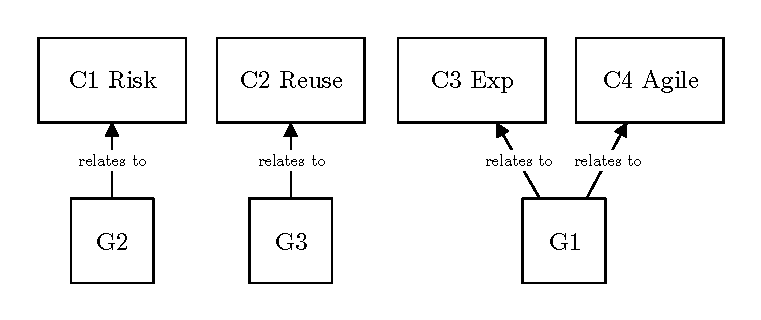
\includegraphics[width=0.75\textwidth]{../figures/req-gaps.pdf}%
\caption{Concept Map of Relationships between Gaps and Requirements}%
\label{fig:req-gaps}%
}
\end{figure}

\begin{gap}{Lack of feasibility with limited resources and limited migration and target environment expertise}{g:1}
Existing \gls{Web Migration} approaches have high requirements with regard to required resources and expertise.
Integration into ongoing, agile development activities is widely overseen with all approaches designed as stand-alone processes requiring dedicated resources.
Feasibility of the approaches with existing staff lacking expertise in target technology and software migration (\cref{c:3} Exp) is only observed for \gls{Encapsulation} approaches and \gls{Transformation} for \glspl{tui}, that have severe drawbacks, as described in \cref{sec:sota.discussion.targets}.
The most promising comprehensive approaches in terms of overall rating (i.e.~REMICS, ARTIST, UWA/UWAT+) all have high expertise requirements.
\end{gap}

\begin{gap}{Lack of demonstration of desirability for decision making and risk management in initial phases}{g:2}
Existing \gls{Web Migration} approaches fail to support decision making in initial phases and address risk.
Their focus is on technical feasibility and financial viability.
Demonstration of desirability of a \glslink{web}{Web}-based version is not considered, leaving decision making without appropriate input specific for the software system to be migrated.
Risk management is hardly addressed.
Risk management techniques focus on technical feasibility studies.
Existing knowledge is not systematically secured against loss during migration beyond stakeholder interviews.
With stakeholders of long-running \glspl{Legacy System} often no longer available, this is not sufficient.
\end{gap}

\begin{gap}{Lack of user interface migration and user interaction reuse}{g:3}
Existing \gls{Web Migration} approaches fail to address user interface aspects of \gls{Web Migration}.
The majority focuses on the backend and does not support migration towards a \glslink{web}{Web}-based user interface.
When regarded, the user interfaces are not native \web user interfaces but terminal user interfaces, or wrappers of graphical desktop user interfaces in the browser.
Reuse of user interaction and continuity of the user interface are neglected.
There are no concrete metrics or tools to achieve a similar ``similar look and feel'' in spite of identified relevance for industry.
\end{gap}
 
To conclude, there are many partial solutions in the \gls{Web Migration} field, but even comprehensive methodologies like ARTIST, REMICS, UWA/UWAT+ exhibit shortcomings in requirements \cref{c:1}, \cref{c:3} and \cref{c:4}, cf. \cref{tbl:eval-overview}, and would benefit from a dedicated solution addressing these gaps.

\vspace{-15pt}
\hypertarget{sec:sota.summary}{%
\section{Summary}\label{sec:sota.summary}}
\vspace{15pt}

This chapter presented relevant standards and a reference model for migration, and assessed existing \gls{Web Migration} approaches according to the requirements elicited in \cref{sec:requirements-analysis}.
A two-dimensional grouping scheme was introduced and a detailed analysis of observations was presented.
This analysis has revealed the lack of a suitable solution combining support of initial phases and \gls{Web Application} target architecture with suitability for \gls{sme}-sized \glspl{isv} in terms of \gls{risk management}, reuse of functionality and user interaction, available expertise and resources, and integration into ongoing agile development.
These shortcomings were synthesized in three main gaps, demonstrating the relevance and need for the solution presented in the following chapter.
The detailed findings have provided input for the creation of the solution concept.

